% Options for packages loaded elsewhere
\PassOptionsToPackage{unicode}{hyperref}
\PassOptionsToPackage{hyphens}{url}
\PassOptionsToPackage{dvipsnames,svgnames,x11names}{xcolor}
%
\documentclass[
  letterpaper,
  DIV=11,
  numbers=noendperiod]{scrartcl}

\usepackage{amsmath,amssymb}
\usepackage{iftex}
\ifPDFTeX
  \usepackage[T1]{fontenc}
  \usepackage[utf8]{inputenc}
  \usepackage{textcomp} % provide euro and other symbols
\else % if luatex or xetex
  \usepackage{unicode-math}
  \defaultfontfeatures{Scale=MatchLowercase}
  \defaultfontfeatures[\rmfamily]{Ligatures=TeX,Scale=1}
\fi
\usepackage{lmodern}
\ifPDFTeX\else  
    % xetex/luatex font selection
  \setmainfont[]{Liberation Serif}
\fi
% Use upquote if available, for straight quotes in verbatim environments
\IfFileExists{upquote.sty}{\usepackage{upquote}}{}
\IfFileExists{microtype.sty}{% use microtype if available
  \usepackage[]{microtype}
  \UseMicrotypeSet[protrusion]{basicmath} % disable protrusion for tt fonts
}{}
\makeatletter
\@ifundefined{KOMAClassName}{% if non-KOMA class
  \IfFileExists{parskip.sty}{%
    \usepackage{parskip}
  }{% else
    \setlength{\parindent}{0pt}
    \setlength{\parskip}{6pt plus 2pt minus 1pt}}
}{% if KOMA class
  \KOMAoptions{parskip=half}}
\makeatother
\usepackage{xcolor}
\setlength{\emergencystretch}{3em} % prevent overfull lines
\setcounter{secnumdepth}{5}
% Make \paragraph and \subparagraph free-standing
\ifx\paragraph\undefined\else
  \let\oldparagraph\paragraph
  \renewcommand{\paragraph}[1]{\oldparagraph{#1}\mbox{}}
\fi
\ifx\subparagraph\undefined\else
  \let\oldsubparagraph\subparagraph
  \renewcommand{\subparagraph}[1]{\oldsubparagraph{#1}\mbox{}}
\fi

\usepackage{color}
\usepackage{fancyvrb}
\newcommand{\VerbBar}{|}
\newcommand{\VERB}{\Verb[commandchars=\\\{\}]}
\DefineVerbatimEnvironment{Highlighting}{Verbatim}{commandchars=\\\{\}}
% Add ',fontsize=\small' for more characters per line
\usepackage{framed}
\definecolor{shadecolor}{RGB}{241,243,245}
\newenvironment{Shaded}{\begin{snugshade}}{\end{snugshade}}
\newcommand{\AlertTok}[1]{\textcolor[rgb]{0.68,0.00,0.00}{#1}}
\newcommand{\AnnotationTok}[1]{\textcolor[rgb]{0.37,0.37,0.37}{#1}}
\newcommand{\AttributeTok}[1]{\textcolor[rgb]{0.40,0.45,0.13}{#1}}
\newcommand{\BaseNTok}[1]{\textcolor[rgb]{0.68,0.00,0.00}{#1}}
\newcommand{\BuiltInTok}[1]{\textcolor[rgb]{0.00,0.23,0.31}{#1}}
\newcommand{\CharTok}[1]{\textcolor[rgb]{0.13,0.47,0.30}{#1}}
\newcommand{\CommentTok}[1]{\textcolor[rgb]{0.37,0.37,0.37}{#1}}
\newcommand{\CommentVarTok}[1]{\textcolor[rgb]{0.37,0.37,0.37}{\textit{#1}}}
\newcommand{\ConstantTok}[1]{\textcolor[rgb]{0.56,0.35,0.01}{#1}}
\newcommand{\ControlFlowTok}[1]{\textcolor[rgb]{0.00,0.23,0.31}{#1}}
\newcommand{\DataTypeTok}[1]{\textcolor[rgb]{0.68,0.00,0.00}{#1}}
\newcommand{\DecValTok}[1]{\textcolor[rgb]{0.68,0.00,0.00}{#1}}
\newcommand{\DocumentationTok}[1]{\textcolor[rgb]{0.37,0.37,0.37}{\textit{#1}}}
\newcommand{\ErrorTok}[1]{\textcolor[rgb]{0.68,0.00,0.00}{#1}}
\newcommand{\ExtensionTok}[1]{\textcolor[rgb]{0.00,0.23,0.31}{#1}}
\newcommand{\FloatTok}[1]{\textcolor[rgb]{0.68,0.00,0.00}{#1}}
\newcommand{\FunctionTok}[1]{\textcolor[rgb]{0.28,0.35,0.67}{#1}}
\newcommand{\ImportTok}[1]{\textcolor[rgb]{0.00,0.46,0.62}{#1}}
\newcommand{\InformationTok}[1]{\textcolor[rgb]{0.37,0.37,0.37}{#1}}
\newcommand{\KeywordTok}[1]{\textcolor[rgb]{0.00,0.23,0.31}{#1}}
\newcommand{\NormalTok}[1]{\textcolor[rgb]{0.00,0.23,0.31}{#1}}
\newcommand{\OperatorTok}[1]{\textcolor[rgb]{0.37,0.37,0.37}{#1}}
\newcommand{\OtherTok}[1]{\textcolor[rgb]{0.00,0.23,0.31}{#1}}
\newcommand{\PreprocessorTok}[1]{\textcolor[rgb]{0.68,0.00,0.00}{#1}}
\newcommand{\RegionMarkerTok}[1]{\textcolor[rgb]{0.00,0.23,0.31}{#1}}
\newcommand{\SpecialCharTok}[1]{\textcolor[rgb]{0.37,0.37,0.37}{#1}}
\newcommand{\SpecialStringTok}[1]{\textcolor[rgb]{0.13,0.47,0.30}{#1}}
\newcommand{\StringTok}[1]{\textcolor[rgb]{0.13,0.47,0.30}{#1}}
\newcommand{\VariableTok}[1]{\textcolor[rgb]{0.07,0.07,0.07}{#1}}
\newcommand{\VerbatimStringTok}[1]{\textcolor[rgb]{0.13,0.47,0.30}{#1}}
\newcommand{\WarningTok}[1]{\textcolor[rgb]{0.37,0.37,0.37}{\textit{#1}}}

\providecommand{\tightlist}{%
  \setlength{\itemsep}{0pt}\setlength{\parskip}{0pt}}\usepackage{longtable,booktabs,array}
\usepackage{calc} % for calculating minipage widths
% Correct order of tables after \paragraph or \subparagraph
\usepackage{etoolbox}
\makeatletter
\patchcmd\longtable{\par}{\if@noskipsec\mbox{}\fi\par}{}{}
\makeatother
% Allow footnotes in longtable head/foot
\IfFileExists{footnotehyper.sty}{\usepackage{footnotehyper}}{\usepackage{footnote}}
\makesavenoteenv{longtable}
\usepackage{graphicx}
\makeatletter
\def\maxwidth{\ifdim\Gin@nat@width>\linewidth\linewidth\else\Gin@nat@width\fi}
\def\maxheight{\ifdim\Gin@nat@height>\textheight\textheight\else\Gin@nat@height\fi}
\makeatother
% Scale images if necessary, so that they will not overflow the page
% margins by default, and it is still possible to overwrite the defaults
% using explicit options in \includegraphics[width, height, ...]{}
\setkeys{Gin}{width=\maxwidth,height=\maxheight,keepaspectratio}
% Set default figure placement to htbp
\makeatletter
\def\fps@figure{htbp}
\makeatother

\usepackage{booktabs}
\usepackage{longtable}
\usepackage{array}
\usepackage{multirow}
\usepackage{wrapfig}
\usepackage{float}
\usepackage{colortbl}
\usepackage{pdflscape}
\usepackage{tabu}
\usepackage{threeparttable}
\usepackage{threeparttablex}
\usepackage[normalem]{ulem}
\usepackage{makecell}
\usepackage{xcolor}
\KOMAoption{captions}{tableheading}
\usepackage{array}
\usepackage{float}
\usepackage{booktabs}
\usepackage{arydshln}
\usepackage{multirow}
\usepackage{xcolor}
\usepackage{tcolorbox}
\usepackage{geometry}
\geometry{left=0.75in, right=0.75in, top=1in, bottom=1in}
\definecolor{pythoncol}{rgb}{0.188,0.412,0.596}
\definecolor{rcol}{rgb}{0.121,0.466,0.705}
\definecolor{bashcol}{rgb}{0.207,0.262,0.392}
\newtcolorbox{pythonheader}{colback=pythoncol!70, colframe=pythoncol, fontupper=\bfseries\color{white}, boxrule=0.1mm, arc=4mm, left=2mm, right=2mm, top=1mm, bottom=1mm, halign=right, sharp corners=south}
\newtcolorbox{rheader}{colback=rcol!70, colframe=rcol, fontupper=\bfseries\color{white}, boxrule=0.1mm, arc=4mm, left=2mm, right=2mm, top=1mm, bottom=1mm, halign=right, sharp corners=south}
\newtcolorbox{bashheader}{colback=bashcol!70, colframe=bashcol, fontupper=\bfseries\color{white}, boxrule=0.1mm, arc=4mm, left=2mm, right=2mm, top=1mm, bottom=1mm, halign=right, sharp corners=south}
\makeatletter
\@ifpackageloaded{caption}{}{\usepackage{caption}}
\AtBeginDocument{%
\ifdefined\contentsname
  \renewcommand*\contentsname{Table of contents}
\else
  \newcommand\contentsname{Table of contents}
\fi
\ifdefined\listfigurename
  \renewcommand*\listfigurename{List of Figures}
\else
  \newcommand\listfigurename{List of Figures}
\fi
\ifdefined\listtablename
  \renewcommand*\listtablename{List of Tables}
\else
  \newcommand\listtablename{List of Tables}
\fi
\ifdefined\figurename
  \renewcommand*\figurename{Figure}
\else
  \newcommand\figurename{Figure}
\fi
\ifdefined\tablename
  \renewcommand*\tablename{Table}
\else
  \newcommand\tablename{Table}
\fi
}
\@ifpackageloaded{float}{}{\usepackage{float}}
\floatstyle{ruled}
\@ifundefined{c@chapter}{\newfloat{codelisting}{h}{lop}}{\newfloat{codelisting}{h}{lop}[chapter]}
\floatname{codelisting}{Listing}
\newcommand*\listoflistings{\listof{codelisting}{List of Listings}}
\makeatother
\makeatletter
\makeatother
\makeatletter
\@ifpackageloaded{caption}{}{\usepackage{caption}}
\@ifpackageloaded{subcaption}{}{\usepackage{subcaption}}
\makeatother
\ifLuaTeX
  \usepackage{selnolig}  % disable illegal ligatures
\fi
\usepackage{bookmark}

\IfFileExists{xurl.sty}{\usepackage{xurl}}{} % add URL line breaks if available
\urlstyle{same} % disable monospaced font for URLs
\hypersetup{
  pdftitle={Genomic-Benchmarks Test},
  colorlinks=true,
  linkcolor={blue},
  filecolor={Maroon},
  citecolor={Blue},
  urlcolor={Blue},
  pdfcreator={LaTeX via pandoc}}

\title{Genomic-Benchmarks Test}
\author{}
\date{}

\begin{document}
\maketitle

\renewcommand*\contentsname{Table of contents}
{
\hypersetup{linkcolor=}
\setcounter{tocdepth}{3}
\tableofcontents
}
\section{Downloading data}\label{downloading-data}

\begin{pythonheader}
Python Code
\end{pythonheader}

\begin{Shaded}
\begin{Highlighting}[]
\CommentTok{\# Listing available datasets}
\ImportTok{from}\NormalTok{ genomic\_benchmarks.data\_check }\ImportTok{import}\NormalTok{ list\_datasets}
\NormalTok{list\_datasets()}
\CommentTok{\# Inspecting each dataset to select two}
\ImportTok{from}\NormalTok{ genomic\_benchmarks.data\_check }\ImportTok{import}\NormalTok{ info }\ImportTok{as}\NormalTok{ info\_gb}
\NormalTok{info\_gb(}\StringTok{"human\_nontata\_promoters"}\NormalTok{) }\CommentTok{\# \textless{}{-} This one will be used}
\NormalTok{info\_gb(}\StringTok{"human\_ensembl\_regulatory"}\NormalTok{)}
\NormalTok{info\_gb(}\StringTok{"human\_enhancers\_cohn"}\NormalTok{)    }\CommentTok{\# \textless{}{-} This one will also be used}
\NormalTok{info\_gb(}\StringTok{"human\_enhancers\_ensembl"}\NormalTok{)}
\CommentTok{\# Downloading datasets}
\ImportTok{from}\NormalTok{ genomic\_benchmarks.loc2seq }\ImportTok{import}\NormalTok{ download\_dataset}
\ImportTok{import}\NormalTok{ os}
\NormalTok{os.chdir(}\StringTok{"/home/davidfm/Projects/UBMI{-}IFC/EnhaProm/datasets/GenomicBenchmarks"}\NormalTok{)}
\NormalTok{download\_dataset(}\StringTok{"human\_nontata\_promoters"}\NormalTok{, version}\OperatorTok{=}\DecValTok{0}\NormalTok{) }
\NormalTok{download\_dataset(}\StringTok{"human\_enhancers\_cohn"}\NormalTok{, version}\OperatorTok{=}\DecValTok{0}\NormalTok{) }
\end{Highlighting}
\end{Shaded}

\section{Formatting data}\label{formatting-data}

The downloaded data came in the form of two directories with many
\emph{.txt} files inside, and seeing that at least `\emph{getShape()}'
function from `\emph{DNAshapeR}' library required FASTA files to work
and it felt right to collect all sequences in a single file, I
transfered all sequences of each cis-regulatory element to their single
respective FASTA file and gave them a simple header.

\begin{bashheader}
Bash Code
\end{bashheader}

\begin{Shaded}
\begin{Highlighting}[]
\BuiltInTok{cd}\NormalTok{ /home/davidfm/Projects/UBMI{-}IFC/EnhaProm/datasets/GenomicBenchmarks/}
\FunctionTok{awk} \StringTok{\textquotesingle{}BEGIN\{counter=0\}\{print "\textgreater{}promoter\_"counter"|train|positive";}
\StringTok{     print $0; counter+=1\}\textquotesingle{}}\NormalTok{ human\_nontata\_promoters/train/positive/}\PreprocessorTok{*}\NormalTok{.txt }\DataTypeTok{\textbackslash{}}
     \OperatorTok{\textgreater{}}\NormalTok{ promoters\_train\_positive.fasta}
\FunctionTok{awk} \StringTok{\textquotesingle{}BEGIN\{counter=0\}\{print "\textgreater{}enhancer\_"counter"|train|positive"; }
\StringTok{     print $0; counter+=1\}\textquotesingle{}}\NormalTok{ human\_enhancers\_cohn/train/positive/}\PreprocessorTok{*}\NormalTok{.txt }\DataTypeTok{\textbackslash{}}
     \OperatorTok{\textgreater{}}\NormalTok{ enhancers\_train\_positive.fasta}
\end{Highlighting}
\end{Shaded}

\section{Libraries used}\label{libraries-used}

Here is a list of the R libraries used for the following analysis, as
well as a reference to my own functions to be used in the
characterization step.

\begin{rheader}
R Code
\end{rheader}

\begin{Shaded}
\begin{Highlighting}[]
\CommentTok{\# For genome{-}functions.R}
\FunctionTok{library}\NormalTok{(stringr)}
\FunctionTok{library}\NormalTok{(stringi)}
\FunctionTok{library}\NormalTok{(primes)}
\CommentTok{\# For parallel computing}
\FunctionTok{library}\NormalTok{(doParallel)}
\FunctionTok{library}\NormalTok{(foreach)}
\CommentTok{\# For biological functions: }
\CommentTok{\#   {-} Local/Global alignments }
\CommentTok{\#   {-} DNA Shape computing}
\FunctionTok{library}\NormalTok{(Biostrings)}
\FunctionTok{library}\NormalTok{(DNAshapeR)}
\CommentTok{\# For plotting}
\FunctionTok{library}\NormalTok{(ggplot2)}
\FunctionTok{library}\NormalTok{(dplyr)}
\FunctionTok{library}\NormalTok{(plyr)}
\CommentTok{\# For pretty tables}
\FunctionTok{library}\NormalTok{(knitr)}
\FunctionTok{library}\NormalTok{(kableExtra)}
\CommentTok{\# For my own functions}
\FunctionTok{source}\NormalTok{(}\StringTok{"/home/davidfm/Projects/UBMI{-}IFC/EnhaProm/scripts/genome{-}functions.R"}\NormalTok{)}
\end{Highlighting}
\end{Shaded}

\section{Characterizing sequences}\label{characterizing-sequences}

Here, we characterize a subset from each of our datasets: 1638 sequences
per regulatory element; 3276 in total. However, there's a circumstance
about the sequences that has to be noted:

\begin{itemize}
\tightlist
\item
  Both datasets have considerably different elements lengthwise:

  \begin{enumerate}
  \def\labelenumi{\arabic{enumi}.}
  \tightlist
  \item
    All promoters have a length of 251 nucleotides.
  \item
    All enhancers have a length of 500 nucleotides.
  \end{enumerate}
\end{itemize}

\begin{Shaded}
\begin{Highlighting}[]
\CommentTok{\# Scanning sequences}
\NormalTok{prom\_fasta }\OtherTok{\textless{}{-}} \StringTok{"datasets/GenomicBenchmarks/promoters\_train\_positive.fasta"}
\NormalTok{enha\_fasta }\OtherTok{\textless{}{-}} \StringTok{"datasets/GenomicBenchmarks/enhancers\_train\_positive.fasta"}
\NormalTok{prom\_seqs }\OtherTok{\textless{}{-}} \FunctionTok{scan}\NormalTok{(prom\_fasta, }\FunctionTok{character}\NormalTok{(), }\AttributeTok{quote =} \StringTok{""}\NormalTok{)[}\FunctionTok{seq}\NormalTok{(}\DecValTok{2}\NormalTok{, }\DecValTok{29484}\NormalTok{, }\DecValTok{2}\NormalTok{)]}
\NormalTok{enha\_seqs }\OtherTok{\textless{}{-}} \FunctionTok{scan}\NormalTok{(enha\_fasta, }\FunctionTok{character}\NormalTok{(), }\AttributeTok{quote =} \StringTok{""}\NormalTok{)[}\FunctionTok{seq}\NormalTok{(}\DecValTok{2}\NormalTok{, }\DecValTok{20842}\NormalTok{, }\DecValTok{2}\NormalTok{)]}
\end{Highlighting}
\end{Shaded}

Given some previous tests done to `sequences\_characterizer()' I came to
the conclusion that parallel computing might provide a higher and more
complex set of data in a feasible time span.

\begin{Shaded}
\begin{Highlighting}[]
\CommentTok{\# Prepairing clusters for parallel computing}
\NormalTok{corescluster }\OtherTok{\textless{}{-}} \FunctionTok{makeCluster}\NormalTok{(}\DecValTok{6}\NormalTok{)}
\FunctionTok{registerDoParallel}\NormalTok{(corescluster)}
\CommentTok{\# Characterizing sequences and exporting to CSV}
\NormalTok{list\_seqs }\OtherTok{\textless{}{-}} \FunctionTok{list}\NormalTok{(}\AttributeTok{promoters =}\NormalTok{ prom\_seqs, }\AttributeTok{enhancers =}\NormalTok{ enha\_seqs)}
\NormalTok{reg\_elems }\OtherTok{\textless{}{-}} \FunctionTok{c}\NormalTok{(}\StringTok{"promoters"}\NormalTok{, }\StringTok{"enhancers"}\NormalTok{)}
\ControlFlowTok{for}\NormalTok{ (reg\_elem }\ControlFlowTok{in}\NormalTok{ reg\_elems) \{}
  \FunctionTok{foreach}\NormalTok{(}\AttributeTok{i =} \DecValTok{1}\SpecialCharTok{:}\DecValTok{6}\NormalTok{) }\SpecialCharTok{\%dopar\%}\NormalTok{ \{}
    \FunctionTok{library}\NormalTok{(stringr) }\CommentTok{\# for some reason we have to specify for}
    \FunctionTok{library}\NormalTok{(stringi) }\CommentTok{\# all the libraries that the sequence}
    \FunctionTok{library}\NormalTok{(primes)  }\CommentTok{\# characterizer needs}
\NormalTok{    i\_start }\OtherTok{\textless{}{-}}\NormalTok{ ((i }\SpecialCharTok{{-}} \DecValTok{1}\NormalTok{) }\SpecialCharTok{*} \DecValTok{273}\NormalTok{) }\SpecialCharTok{+} \DecValTok{1}
\NormalTok{    i\_final }\OtherTok{\textless{}{-}}\NormalTok{ i }\SpecialCharTok{*} \DecValTok{273}
    \ControlFlowTok{if}\NormalTok{ (i }\SpecialCharTok{\textgreater{}} \DecValTok{1}\NormalTok{) \{     }\CommentTok{\# Conditional so that only the first CSV has headers}
      \FunctionTok{write.table}\NormalTok{(}\FunctionTok{sequences\_characterizer}\NormalTok{(list\_seqs[[reg\_elem]][i\_start}\SpecialCharTok{:}\NormalTok{i\_final],}
                                          \AttributeTok{k\_max =} \DecValTok{6}\NormalTok{, }\AttributeTok{optim =} \ConstantTok{TRUE}\NormalTok{),}
                  \FunctionTok{paste}\NormalTok{(}\StringTok{"datasets/GB{-}Testing/test"}\NormalTok{, reg\_elem, }\StringTok{"{-}minitraining\_"}\NormalTok{,}
\NormalTok{                        i, }\StringTok{".csv"}\NormalTok{, }\AttributeTok{sep =} \StringTok{""}\NormalTok{), }\AttributeTok{sep =} \StringTok{","}\NormalTok{,}
                  \AttributeTok{row.names =} \ConstantTok{FALSE}\NormalTok{, }\AttributeTok{col.names =} \ConstantTok{FALSE}\NormalTok{)}
\NormalTok{    \} }\ControlFlowTok{else}\NormalTok{ \{}
      \FunctionTok{write.csv}\NormalTok{(}\FunctionTok{sequences\_characterizer}\NormalTok{(list\_seqs[[reg\_elem]][i\_start}\SpecialCharTok{:}\NormalTok{i\_final],}
                                        \AttributeTok{k\_max =} \DecValTok{6}\NormalTok{, }\AttributeTok{optim =} \ConstantTok{TRUE}\NormalTok{),}
                \FunctionTok{paste}\NormalTok{(}\StringTok{"datasets/GB{-}Testing/"}\NormalTok{, reg\_elem, }\StringTok{"{-}minitraining\_"}\NormalTok{,}
\NormalTok{                      i, }\StringTok{".csv"}\NormalTok{, }\AttributeTok{sep =} \StringTok{""}\NormalTok{), }\AttributeTok{row.names =} \ConstantTok{FALSE}\NormalTok{)}
\NormalTok{    \}}
\NormalTok{  \}}
\NormalTok{\}}
\end{Highlighting}
\end{Shaded}

\section{Concatenating CSV's}\label{concatenating-csvs}

It was decided to produce many files instead of appending over the same
CSV table in order to apply a sort of quality control checkup after the
parallel computing was done. This, because when forcing the process RAM
overload was possible and the function could die mid-process. Since our
data was separated in six tables per cis-regulatory element, here we
only join each set together in a single CSV.

\begin{bashheader}
Bash Code
\end{bashheader}

\begin{Shaded}
\begin{Highlighting}[]
\FunctionTok{cat}\NormalTok{ datasets/GB{-}Testing/testpromoters{-}minitraining\_}\PreprocessorTok{*}\NormalTok{.csv }\DataTypeTok{\textbackslash{}}
    \OperatorTok{\textgreater{}}\NormalTok{ datasets/GB{-}Testing/test{-}1638{-}promoters{-}6mers.csv}
\FunctionTok{cat}\NormalTok{ datasets/GB{-}Testing/testenhancers{-}minitraining\_}\PreprocessorTok{*}\NormalTok{.csv }\DataTypeTok{\textbackslash{}}
    \OperatorTok{\textgreater{}}\NormalTok{ datasets/GB{-}Testing/test{-}1638{-}enhancers{-}6mers.csv}
\end{Highlighting}
\end{Shaded}

\section{Data description}\label{data-description}

\newcolumntype{L}[1]{>{\raggedright\arraybackslash}p{#1}}
\newcolumntype{C}[1]{>{\centering\arraybackslash}p{#1}}
\newcolumntype{M}[1]{>{\centering\arraybackslash}m{#1}}
\newcolumntype{R}[1]{>{\raggedleft\arraybackslash}p{#1}}

\begin{table}[H]
\caption{Overview of each column generated by '\textit{sequences-characterizer()}'}
\centering
% Using the new column types L, C, and R for custom width and orientation
\begin{tabular}{|L{2.5cm}|C{4cm}|C{5cm}|} 
\hline
\centering \textbf{Column} & \textbf{Description} & \textbf{Section Processed} \\
\hline
A & \parbox[c][1.2cm]{4cm}{\centering Percentage of Alanines} & \multirow{6}{*}{\underline{per Sequence}} \\
\cdashline{1-2}
T & \parbox[c][1.2cm]{4cm}{\setlength\parindent{4pt}Percentage of Thymines} & \\
\cdashline{1-2}
C & \parbox[c][1.2cm]{4cm}{\centering Percentage of Cytosines} & \\
\cdashline{1-2}
G & \parbox[c][1.2cm]{4cm}{\centering Percentage of Guanines} & \\
\cdashline{1-2}
temp & \parbox[c][1.2cm]{4cm}{\centering Melting Temperature} & \\
\cdashline{1-2}
shan & \parbox[c][1.2cm]{4cm}{\centering Shannon Coefficient} & \\
\hline
kN.M\_prod & \parbox[c][1.25cm]{4cm}{\centering KSG Product} & \multirow{4}{*}{\parbox[t]{8cm}{
\setlength\parindent{45pt}\underline{per Kmer:}\\\\
each possible kmer of size N\\
is identified on a scale of 1 to\\
$4^N$ denoted by M.\\\\
\texttt{
i.e. k3.1 (or the first\\
kmer of size 3) would be\\
AAA; k4.2 would be AAAC\\
}
}} \\
\cdashline{1-2}
kN.M\_barc & \parbox[c][1.2cm]{4cm}{\centering Barcode Profile} & \\
\cdashline{1-2}
kN.M\_pals & \parbox[c][1.2cm]{4cm}{\centering Palindrome Profile} & \\
\cdashline{1-2}
kN.M\_revc & \parbox[c][1.7cm]{4cm}{\centering Reverse Complement Profile} & \\
\hline
\end{tabular}
\end{table}

Prior to our primary analysis, it feels reasonable to explain the
columns per sequence produced by our tabulator
`\emph{sequences\_characterizer()}'. From here we'll first describe the
ones computed sequence-wise, the ones computed kmer-wise, then the ones
computed over each kmer distribution, and finally the ones corresponding
to DNA-Shape; this feature comes at last considering `\emph{getShape()}'
function makes its' own dataframe. The ones in \textbf{black} are
already integrated in the table, the ones in \color{red} \textbf{red}
\color{black} are yet to be adjoined:

\underline{Per sequence}

\begin{itemize}
\tightlist
\item
  From \emph{`genome-functions.R'}:

  \begin{itemize}
  \item
    \textbf{A, T, C, G} - \emph{Nucleotide Percentages} per sequence.
  \item
    \textbf{temp} - \textit{Melting \underline{Temp}erature}:
    Temperature at which DNA's double helix dissociates into single
    strands. \emph{It's dependent on GC percentage and sequence length.}
  \item
    \textbf{shan} - \textit{\underline{Shan}non Entropy Coefficient}:
    Statistical quantifier of information in a system. Measures the
    uncertainty a set of data has. In this case is a
    nucleotide-diversity metric. \emph{It's dependent on nucleotide
    percentages.}
  \end{itemize}
\item
  From \emph{`Biostrings'}:

  \begin{itemize}
  \item
    \color{red}\textbf{la\_sc} \color{black} -
    \textit{\underline{L}ocal \underline{A}lignment \underline{Sc}ore}
  \item
    \color{red}\textbf{la\_id} \color{black} -
    \textit{\underline{L}ocal \underline{A}lignment \underline{Id}entity}
  \item
    \color{red}\textbf{ga\_sc} \color{black} -
    \textit{\underline{G}lobal \underline{A}lignment \underline{Sc}ore}
  \item
    \color{red}\textbf{ga\_id} \color{black} -
    \textit{\underline{G}lobal \underline{A}lignment \underline{Id}entity}
  \end{itemize}
\end{itemize}

\underline{Per kmer} \newfontfamily\mynimbus{Nimbus Sans Narrow}

\begin{itemize}
\item
  From \emph{`genome-functions.R'}:

  \begin{itemize}
  \item
    \textbf{kN.M\_prod} - \textit{KSG \underline{Prod}uct}: Its obtained
    by multiplying \mynimbus\textbf{
    \underline{K}mer-Percentage * \underline{S}hannon Entropy * \underline{G}C-Percentage}
    \fontspec{Liberation Serif} (in concept). However, this is a little
    tricky since you don't want the product to be zero if a sequence is
    solely composed of A/T nucleotides.
  \item
    \textbf{kN.M\_barc} - \textit{\underline{Barc}ode Profile}:
  \item
    \textbf{kN.M\_pals} -
    \textit{\underline{Pal}indrome\underline{s}' Profile}:
  \item
    \textbf{kN.M\_revc} -
    \textit{\underline{Rev}erse \underline{C}omplement Profile}:
  \end{itemize}
\end{itemize}

\underline{Per kmer distribution}

\underline{Per non-defined kmer}

\begin{itemize}
\item
  From \emph{`DNAshapeR'}: \newline Its produced a row per sequence and
  a set vectors (EP, MGW, HelT, Roll \& ProT as default) obtained when
  dividing each sequence in kmers (length non-defined by me) of whose
  length depends on sequence-length, so I would classify it as per

  \begin{itemize}
  \item
    \color{red}\textbf{sh\_ep} \color{black} - Shape EP
  \item
    \color{red}\textbf{sh\_mgw} \color{black} - Shape MGW
  \item
    \color{red}\textbf{sh\_helt} \color{black} - Shape HelT
  \item
    \color{red}\textbf{sh\_roll} \color{black} - Shape Roll
  \item
    \color{red}\textbf{sh\_prot} \color{black} - Shape ProT
  \end{itemize}
\end{itemize}

\section{Primary analysis}\label{primary-analysis}

Firstly we read our CSV tables into our conviniently named dataframes.

We could have concatenated both tables together, however I prefer to
keep them in different files.

\begin{rheader}
R Code
\end{rheader}

\begin{Shaded}
\begin{Highlighting}[]
\FunctionTok{setwd}\NormalTok{(}\StringTok{"/home/davidfm/Projects/UBMI{-}IFC/EnhaProm"}\NormalTok{)}
\NormalTok{testpromoters }\OtherTok{\textless{}{-}} \FunctionTok{read.csv}\NormalTok{(}\StringTok{"datasets/GB{-}Testing/test{-}1638{-}promoters{-}6mers.csv"}\NormalTok{, }
                          \AttributeTok{check.names =}\NormalTok{ F)}
\NormalTok{testenhancers }\OtherTok{\textless{}{-}} \FunctionTok{read.csv}\NormalTok{(}\StringTok{"datasets/GB{-}Testing/test{-}1638{-}enhancers{-}6mers.csv"}\NormalTok{, }
                          \AttributeTok{check.names =}\NormalTok{ F)}
\end{Highlighting}
\end{Shaded}

First we get an overviwew of the dimensions of our data:

\begin{Shaded}
\begin{Highlighting}[]
\FunctionTok{deparse}\NormalTok{(}\FunctionTok{substitute}\NormalTok{(testpromoters))}
\FunctionTok{deparse}\NormalTok{(}\FunctionTok{substitute}\NormalTok{(testenhancers))}
\FunctionTok{dim}\NormalTok{(testpromoters)}
\FunctionTok{dim}\NormalTok{(testenhancers)}
\end{Highlighting}
\end{Shaded}

\begin{figure}

\begin{minipage}{0.50\linewidth}

\begin{verbatim}
[1] "testpromoters"
\end{verbatim}

\end{minipage}%
%
\begin{minipage}{0.50\linewidth}

\begin{verbatim}
[1] "testenhancers"
\end{verbatim}

\end{minipage}%
\newline
\begin{minipage}{0.50\linewidth}

\begin{verbatim}
[1]  1638 21830
\end{verbatim}

\end{minipage}%
%
\begin{minipage}{0.50\linewidth}

\begin{verbatim}
[1]  1638 21830
\end{verbatim}

\end{minipage}%

\end{figure}%

It's noticeable the fact that we have way more columns than rows in this
test table. Let's get a glimpse of the records corresponding to the
first three promoters.

\begin{Shaded}
\begin{Highlighting}[]
\FunctionTok{kable}\NormalTok{(testpromoters[}\DecValTok{1}\SpecialCharTok{:}\DecValTok{3}\NormalTok{,}\DecValTok{1}\SpecialCharTok{:}\DecValTok{18}\NormalTok{])}
\end{Highlighting}
\end{Shaded}

\begin{longtable}[]{@{}rrrrrr@{}}
\toprule\noalign{}
A & T & C & G & temp & shan \\
\midrule\noalign{}
\endhead
\bottomrule\noalign{}
\endlastfoot
0.1673307 & 0.2231076 & 0.3306773 & 0.2788845 & 87.21315 & 1.956136 \\
0.2629482 & 0.2788845 & 0.2549801 & 0.2031873 & 81.00598 & 1.990374 \\
0.3625498 & 0.2031873 & 0.2470120 & 0.1872510 & 80.02590 & 1.948719 \\
\end{longtable}

\begin{longtable}[]{@{}
  >{\raggedleft\arraybackslash}p{(\columnwidth - 10\tabcolsep) * \real{0.1515}}
  >{\raggedleft\arraybackslash}p{(\columnwidth - 10\tabcolsep) * \real{0.1515}}
  >{\raggedleft\arraybackslash}p{(\columnwidth - 10\tabcolsep) * \real{0.1970}}
  >{\raggedleft\arraybackslash}p{(\columnwidth - 10\tabcolsep) * \real{0.1970}}
  >{\raggedleft\arraybackslash}p{(\columnwidth - 10\tabcolsep) * \real{0.1515}}
  >{\raggedleft\arraybackslash}p{(\columnwidth - 10\tabcolsep) * \real{0.1515}}@{}}
\toprule\noalign{}
\begin{minipage}[b]{\linewidth}\raggedleft
k2.1\_prod
\end{minipage} & \begin{minipage}[b]{\linewidth}\raggedleft
k2.1\_barc
\end{minipage} & \begin{minipage}[b]{\linewidth}\raggedleft
k2.1\_pals
\end{minipage} & \begin{minipage}[b]{\linewidth}\raggedleft
k2.1\_revc
\end{minipage} & \begin{minipage}[b]{\linewidth}\raggedleft
k2.2\_prod
\end{minipage} & \begin{minipage}[b]{\linewidth}\raggedleft
k2.2\_barc
\end{minipage} \\
\midrule\noalign{}
\endhead
\bottomrule\noalign{}
\endlastfoot
9 & 1.959765 & 2.177403e+09 & 1.374020e+12 & 17.11198 & 1.531862 \\
17 & 2.633165 & 1.138401e+17 & 2.971115e+17 & 26.44579 & 2.624612 \\
38 & 5.347025 & 3.981015e+36 & 8.100763e+29 & 24.89016 & 1.855662 \\
\end{longtable}

\begin{longtable}[]{@{}
  >{\raggedleft\arraybackslash}p{(\columnwidth - 10\tabcolsep) * \real{0.1806}}
  >{\raggedleft\arraybackslash}p{(\columnwidth - 10\tabcolsep) * \real{0.1806}}
  >{\raggedleft\arraybackslash}p{(\columnwidth - 10\tabcolsep) * \real{0.1389}}
  >{\raggedleft\arraybackslash}p{(\columnwidth - 10\tabcolsep) * \real{0.1389}}
  >{\raggedleft\arraybackslash}p{(\columnwidth - 10\tabcolsep) * \real{0.1806}}
  >{\raggedleft\arraybackslash}p{(\columnwidth - 10\tabcolsep) * \real{0.1806}}@{}}
\toprule\noalign{}
\begin{minipage}[b]{\linewidth}\raggedleft
k2.2\_pals
\end{minipage} & \begin{minipage}[b]{\linewidth}\raggedleft
k2.2\_revc
\end{minipage} & \begin{minipage}[b]{\linewidth}\raggedleft
k2.3\_prod
\end{minipage} & \begin{minipage}[b]{\linewidth}\raggedleft
k2.3\_barc
\end{minipage} & \begin{minipage}[b]{\linewidth}\raggedleft
k2.3\_pals
\end{minipage} & \begin{minipage}[b]{\linewidth}\raggedleft
k2.3\_revc
\end{minipage} \\
\midrule\noalign{}
\endhead
\bottomrule\noalign{}
\endlastfoot
3.845422e+15 & 3.525451e+11 & 26.44579 & 2.445328 & 4.788062e+13 &
1.305836e+26 \\
2.607331e+20 & 6.308689e+14 & 24.89016 & 2.513656 & 1.320117e+14 &
6.435389e+19 \\
1.156904e+25 & 3.573059e+12 & 34.22397 & 3.431445 & 6.011592e+17 &
7.178542e+17 \\
\end{longtable}

Let's get a glimpse of the records corresponding to the first three
enhancers.

\begin{Shaded}
\begin{Highlighting}[]
\FunctionTok{kable}\NormalTok{(testenhancers[}\DecValTok{1}\SpecialCharTok{:}\DecValTok{3}\NormalTok{,}\DecValTok{1}\SpecialCharTok{:}\DecValTok{18}\NormalTok{])}
\end{Highlighting}
\end{Shaded}

\begin{longtable}[]{@{}rrrrrr@{}}
\toprule\noalign{}
A & T & C & G & temp & shan \\
\midrule\noalign{}
\endhead
\bottomrule\noalign{}
\endlastfoot
0.240 & 0.236 & 0.234 & 0.290 & 85.0392 & 1.993988 \\
0.204 & 0.286 & 0.210 & 0.300 & 84.4652 & 1.978249 \\
0.250 & 0.280 & 0.258 & 0.212 & 82.8252 & 1.992923 \\
\end{longtable}

\begin{longtable}[]{@{}
  >{\raggedleft\arraybackslash}p{(\columnwidth - 10\tabcolsep) * \real{0.1515}}
  >{\raggedleft\arraybackslash}p{(\columnwidth - 10\tabcolsep) * \real{0.1515}}
  >{\raggedleft\arraybackslash}p{(\columnwidth - 10\tabcolsep) * \real{0.1970}}
  >{\raggedleft\arraybackslash}p{(\columnwidth - 10\tabcolsep) * \real{0.1970}}
  >{\raggedleft\arraybackslash}p{(\columnwidth - 10\tabcolsep) * \real{0.1515}}
  >{\raggedleft\arraybackslash}p{(\columnwidth - 10\tabcolsep) * \real{0.1515}}@{}}
\toprule\noalign{}
\begin{minipage}[b]{\linewidth}\raggedleft
k2.1\_prod
\end{minipage} & \begin{minipage}[b]{\linewidth}\raggedleft
k2.1\_barc
\end{minipage} & \begin{minipage}[b]{\linewidth}\raggedleft
k2.1\_pals
\end{minipage} & \begin{minipage}[b]{\linewidth}\raggedleft
k2.1\_revc
\end{minipage} & \begin{minipage}[b]{\linewidth}\raggedleft
k2.2\_prod
\end{minipage} & \begin{minipage}[b]{\linewidth}\raggedleft
k2.2\_barc
\end{minipage} \\
\midrule\noalign{}
\endhead
\bottomrule\noalign{}
\endlastfoot
36 & 10.432345 & 1.885437e+37 & 8.632413e+30 & 24.89016 & 6.027803 \\
20 & 6.153015 & 5.673403e+20 & 1.061673e+53 & 23.33452 & 4.984254 \\
31 & 9.936447 & 1.640775e+32 & 5.563175e+39 & 46.66905 & 9.301359 \\
\end{longtable}

\begin{longtable}[]{@{}
  >{\raggedleft\arraybackslash}p{(\columnwidth - 10\tabcolsep) * \real{0.1806}}
  >{\raggedleft\arraybackslash}p{(\columnwidth - 10\tabcolsep) * \real{0.1806}}
  >{\raggedleft\arraybackslash}p{(\columnwidth - 10\tabcolsep) * \real{0.1389}}
  >{\raggedleft\arraybackslash}p{(\columnwidth - 10\tabcolsep) * \real{0.1389}}
  >{\raggedleft\arraybackslash}p{(\columnwidth - 10\tabcolsep) * \real{0.1806}}
  >{\raggedleft\arraybackslash}p{(\columnwidth - 10\tabcolsep) * \real{0.1806}}@{}}
\toprule\noalign{}
\begin{minipage}[b]{\linewidth}\raggedleft
k2.2\_pals
\end{minipage} & \begin{minipage}[b]{\linewidth}\raggedleft
k2.2\_revc
\end{minipage} & \begin{minipage}[b]{\linewidth}\raggedleft
k2.3\_prod
\end{minipage} & \begin{minipage}[b]{\linewidth}\raggedleft
k2.3\_barc
\end{minipage} & \begin{minipage}[b]{\linewidth}\raggedleft
k2.3\_pals
\end{minipage} & \begin{minipage}[b]{\linewidth}\raggedleft
k2.3\_revc
\end{minipage} \\
\midrule\noalign{}
\endhead
\bottomrule\noalign{}
\endlastfoot
1.579134e+29 & 1.707234e+31 & 76.22611 & 13.43518 & 3.557032e+41 &
5.830130e+44 \\
4.485619e+32 & 1.810188e+35 & 73.11484 & 13.29662 & 3.273426e+39 &
3.755909e+39 \\
9.951038e+37 & 3.612544e+25 & 60.66976 & 12.53356 & 4.255600e+33 &
3.010280e+57 \\
\end{longtable}

\begin{Shaded}
\begin{Highlighting}[]
\NormalTok{meanpromoters }\OtherTok{\textless{}{-}} \FunctionTok{colMeans}\NormalTok{(testpromoters)}
\NormalTok{meanenhancers }\OtherTok{\textless{}{-}} \FunctionTok{colMeans}\NormalTok{(testenhancers)}
\NormalTok{sdpromoters }\OtherTok{\textless{}{-}} \FunctionTok{apply}\NormalTok{(testpromoters, }\DecValTok{2}\NormalTok{, sd)}
\NormalTok{sdenhancers }\OtherTok{\textless{}{-}} \FunctionTok{apply}\NormalTok{(testenhancers, }\DecValTok{2}\NormalTok{, sd)}
\CommentTok{\# names\_test \textless{}{-} rep(names(testpromoters),2)}
\NormalTok{cre\_summary }\OtherTok{\textless{}{-}} \FunctionTok{data.frame}\NormalTok{(}\AttributeTok{Type =} \FunctionTok{factor}\NormalTok{(}\FunctionTok{rep}\NormalTok{(}\FunctionTok{c}\NormalTok{(}\StringTok{"Promoter"}\NormalTok{,}\StringTok{"Enhancer"}\NormalTok{), }
                                        \AttributeTok{each =} \FunctionTok{length}\NormalTok{(testpromoters))),}
                          \AttributeTok{Field =} \FunctionTok{rep}\NormalTok{(}\FunctionTok{names}\NormalTok{(testpromoters),}\DecValTok{2}\NormalTok{),}
                          \AttributeTok{Means =} \FunctionTok{c}\NormalTok{(meanpromoters, meanenhancers),}
                          \AttributeTok{StDevs =} \FunctionTok{c}\NormalTok{(sdpromoters, sdenhancers))}
\CommentTok{\# head(cre\_summary)}
\FunctionTok{kable}\NormalTok{(cre\_summary[}\FunctionTok{c}\NormalTok{(}\DecValTok{1}\SpecialCharTok{:}\DecValTok{10}\NormalTok{,}\DecValTok{21831}\SpecialCharTok{:}\DecValTok{21840}\NormalTok{),])}
\end{Highlighting}
\end{Shaded}

\begin{longtable}[]{@{}lllrr@{}}
\toprule\noalign{}
& Type & Field & Means & StDevs \\
\midrule\noalign{}
\endhead
\bottomrule\noalign{}
\endlastfoot
1 & Promoter & A & 1.911256e-01 & 7.145510e-02 \\
2 & Promoter & T & 1.995826e-01 & 7.599340e-02 \\
3 & Promoter & C & 2.962655e-01 & 8.067840e-02 \\
4 & Promoter & G & 3.130263e-01 & 8.524230e-02 \\
5 & Promoter & temp & 8.720208e+01 & 5.379461e+00 \\
6 & Promoter & shan & 1.891724e+00 & 9.437000e-02 \\
7 & Promoter & k2.1\_prod & 1.196276e+01 & 8.995306e+00 \\
8 & Promoter & k2.1\_barc & 1.500971e+00 & 1.229003e+00 \\
9 & Promoter & k2.1\_pals & 2.634405e+51 & 1.065029e+53 \\
10 & Promoter & k2.1\_revc & 9.789346e+62 & 3.960331e+64 \\
21831 & Enhancer & A & 2.653712e-01 & 5.853000e-02 \\
21832 & Enhancer & T & 2.678205e-01 & 5.815610e-02 \\
21833 & Enhancer & C & 2.351111e-01 & 5.648440e-02 \\
21834 & Enhancer & G & 2.316972e-01 & 5.435370e-02 \\
21835 & Enhancer & temp & 8.269434e+01 & 3.785299e+00 \\
21836 & Enhancer & shan & 1.959202e+00 & 3.892580e-02 \\
21837 & Enhancer & k2.1\_prod & 4.093346e+01 & 1.835697e+01 \\
21838 & Enhancer & k2.1\_barc & 1.208127e+01 & 5.751107e+00 \\
21839 & Enhancer & k2.1\_pals & 2.567318e+112 & 1.038419e+114 \\
21840 & Enhancer & k2.1\_revc & 3.321646e+121 & 1.344343e+123 \\
\end{longtable}

\begin{Shaded}
\begin{Highlighting}[]
\CommentTok{\# Get only \textquotesingle{}prod\textquotesingle{} columns of each kmer}
\NormalTok{k2 }\OtherTok{\textless{}{-}} \FunctionTok{n\_ki}\NormalTok{(}\DecValTok{2}\NormalTok{); k3 }\OtherTok{\textless{}{-}} \FunctionTok{n\_ki}\NormalTok{(}\DecValTok{3}\NormalTok{); k4 }\OtherTok{\textless{}{-}} \FunctionTok{n\_ki}\NormalTok{(}\DecValTok{4}\NormalTok{); k5 }\OtherTok{\textless{}{-}} \FunctionTok{n\_ki}\NormalTok{(}\DecValTok{5}\NormalTok{); k6 }\OtherTok{\textless{}{-}} \FunctionTok{n\_ki}\NormalTok{(}\DecValTok{6}\NormalTok{) }
\NormalTok{kmer\_sections\_indexes }\OtherTok{\textless{}{-}} \FunctionTok{c}\NormalTok{(}\DecValTok{1}\NormalTok{, }
\NormalTok{                           k2, }
\NormalTok{                           k2 }\SpecialCharTok{+} \DecValTok{1}\NormalTok{, }
\NormalTok{                           k2 }\SpecialCharTok{+}\NormalTok{ k3, }
\NormalTok{                           k2 }\SpecialCharTok{+}\NormalTok{ k3 }\SpecialCharTok{+} \DecValTok{1}\NormalTok{,}
\NormalTok{                           k2 }\SpecialCharTok{+}\NormalTok{ k3 }\SpecialCharTok{+}\NormalTok{ k4, }
\NormalTok{                           k2 }\SpecialCharTok{+}\NormalTok{ k3 }\SpecialCharTok{+}\NormalTok{ k4 }\SpecialCharTok{+} \DecValTok{1}\NormalTok{,}
\NormalTok{                           k2 }\SpecialCharTok{+}\NormalTok{ k3 }\SpecialCharTok{+}\NormalTok{ k4 }\SpecialCharTok{+}\NormalTok{ k5, }
\NormalTok{                           k2 }\SpecialCharTok{+}\NormalTok{ k3 }\SpecialCharTok{+}\NormalTok{ k4 }\SpecialCharTok{+}\NormalTok{ k5 }\SpecialCharTok{+} \DecValTok{1}\NormalTok{, }
\NormalTok{                           k2 }\SpecialCharTok{+}\NormalTok{ k3 }\SpecialCharTok{+}\NormalTok{ k4 }\SpecialCharTok{+}\NormalTok{ k5 }\SpecialCharTok{+}\NormalTok{ k6)}
\NormalTok{prod\_indexes }\OtherTok{\textless{}{-}} \FunctionTok{seq}\NormalTok{(}\DecValTok{7}\NormalTok{,}\DecValTok{21827}\NormalTok{,}\DecValTok{4}\NormalTok{)}
\NormalTok{barc\_indexes }\OtherTok{\textless{}{-}} \FunctionTok{seq}\NormalTok{(}\DecValTok{8}\NormalTok{,}\DecValTok{21828}\NormalTok{,}\DecValTok{4}\NormalTok{)}
\NormalTok{pals\_indexes }\OtherTok{\textless{}{-}} \FunctionTok{seq}\NormalTok{(}\DecValTok{9}\NormalTok{,}\DecValTok{21829}\NormalTok{,}\DecValTok{4}\NormalTok{)}
\NormalTok{revc\_indexes }\OtherTok{\textless{}{-}} \FunctionTok{seq}\NormalTok{(}\DecValTok{10}\NormalTok{,}\DecValTok{21830}\NormalTok{,}\DecValTok{4}\NormalTok{)}
\NormalTok{all\_prod\_indexes }\OtherTok{\textless{}{-}} \FunctionTok{c}\NormalTok{(prod\_indexes, }\DecValTok{21830} \SpecialCharTok{+}\NormalTok{ prod\_indexes)}
\NormalTok{all\_barc\_indexes }\OtherTok{\textless{}{-}} \FunctionTok{c}\NormalTok{(barc\_indexes, }\DecValTok{21830} \SpecialCharTok{+}\NormalTok{ barc\_indexes)}
\NormalTok{all\_pals\_indexes }\OtherTok{\textless{}{-}} \FunctionTok{c}\NormalTok{(pals\_indexes, }\DecValTok{21830} \SpecialCharTok{+}\NormalTok{ pals\_indexes)}
\NormalTok{all\_revc\_indexes }\OtherTok{\textless{}{-}} \FunctionTok{c}\NormalTok{(revc\_indexes, }\DecValTok{21830} \SpecialCharTok{+}\NormalTok{ revc\_indexes)}
\FunctionTok{kable}\NormalTok{(}\FunctionTok{head}\NormalTok{(testenhancers[, barc\_indexes])[,}\FunctionTok{c}\NormalTok{(}\DecValTok{1}\SpecialCharTok{:}\DecValTok{8}\NormalTok{,}\FunctionTok{length}\NormalTok{(barc\_indexes))])}
\end{Highlighting}
\end{Shaded}

\begin{longtable}[]{@{}
  >{\raggedleft\arraybackslash}p{(\columnwidth - 16\tabcolsep) * \real{0.1075}}
  >{\raggedleft\arraybackslash}p{(\columnwidth - 16\tabcolsep) * \real{0.1075}}
  >{\raggedleft\arraybackslash}p{(\columnwidth - 16\tabcolsep) * \real{0.1075}}
  >{\raggedleft\arraybackslash}p{(\columnwidth - 16\tabcolsep) * \real{0.1075}}
  >{\raggedleft\arraybackslash}p{(\columnwidth - 16\tabcolsep) * \real{0.1075}}
  >{\raggedleft\arraybackslash}p{(\columnwidth - 16\tabcolsep) * \real{0.1075}}
  >{\raggedleft\arraybackslash}p{(\columnwidth - 16\tabcolsep) * \real{0.1075}}
  >{\raggedleft\arraybackslash}p{(\columnwidth - 16\tabcolsep) * \real{0.1075}}
  >{\raggedleft\arraybackslash}p{(\columnwidth - 16\tabcolsep) * \real{0.1398}}@{}}
\toprule\noalign{}
\begin{minipage}[b]{\linewidth}\raggedleft
k2.1\_barc
\end{minipage} & \begin{minipage}[b]{\linewidth}\raggedleft
k2.2\_barc
\end{minipage} & \begin{minipage}[b]{\linewidth}\raggedleft
k2.3\_barc
\end{minipage} & \begin{minipage}[b]{\linewidth}\raggedleft
k2.4\_barc
\end{minipage} & \begin{minipage}[b]{\linewidth}\raggedleft
k2.5\_barc
\end{minipage} & \begin{minipage}[b]{\linewidth}\raggedleft
k2.6\_barc
\end{minipage} & \begin{minipage}[b]{\linewidth}\raggedleft
k2.7\_barc
\end{minipage} & \begin{minipage}[b]{\linewidth}\raggedleft
k2.8\_barc
\end{minipage} & \begin{minipage}[b]{\linewidth}\raggedleft
k6.4096\_barc
\end{minipage} \\
\midrule\noalign{}
\endhead
\bottomrule\noalign{}
\endlastfoot
10.432345 & 6.027803 & 13.435177 & 5.182017 & 9.672032 & 14.452432 &
2.0213095 & 13.731694 & 0.0000000 \\
6.153015 & 4.984254 & 13.296620 & 6.098819 & 10.185028 & 7.732096 &
1.3635487 & 10.150355 & 0.3058662 \\
9.936447 & 9.301359 & 12.533556 & 6.353834 & 10.894642 & 9.025510 &
1.3565393 & 16.335286 & 0.0000000 \\
23.252879 & 8.744180 & 13.868229 & 9.853451 & 12.204317 & 3.958776 &
0.0930320 & 8.444184 & 0.0000000 \\
3.814939 & 7.617881 & 9.290377 & 5.365261 & 10.457174 & 13.017956 &
1.4893074 & 14.727846 & 2.7938687 \\
14.929810 & 6.939986 & 12.525913 & 11.864119 & 10.686542 & 2.227940 &
0.9421584 & 7.264738 & 0.0000000 \\
\end{longtable}

\begin{Shaded}
\begin{Highlighting}[]
\FunctionTok{kable}\NormalTok{(}\FunctionTok{head}\NormalTok{(testenhancers[}\DecValTok{496}\SpecialCharTok{:}\DecValTok{500}\NormalTok{, barc\_indexes], }\DecValTok{5}\NormalTok{)[kmer\_sections\_indexes])}
\end{Highlighting}
\end{Shaded}

\begin{longtable*}[t]{r>{\raggedleft\arraybackslash}p{1in}>{\raggedleft\arraybackslash}p{1in}>{\raggedleft\arraybackslash}p{1in}>{\raggedleft\arraybackslash}p{1in}}
\toprule
k2.1\_barc & k2.16\_barc & k3.1\_barc & k3.64\_barc & k4.1\_barc\\
\midrule
21.956001 & 19.037416 & 10.818389 & 10.1549028 & 4.0524987\\
13.176071 & 24.867054 & 4.338962 & 12.7780698 & 0.7618167\\
17.160666 & 15.872687 & 7.995707 & 5.5079687 & 3.3905390\\
9.811821 & 2.290862 & 3.488092 & 0.6337946 & 1.1768199\\
9.711428 & 9.532818 & 1.272394 & 2.3765456 & 0.0000000\\
\bottomrule
\end{longtable*}

\begin{longtable*}[t]{r>{\raggedleft\arraybackslash}p{1in}>{\raggedleft\arraybackslash}p{1in}>{\raggedleft\arraybackslash}p{1in}>{\raggedleft\arraybackslash}p{1in}}
\toprule
k4.256\_barc & k5.1\_barc & k5.1024\_barc & k6.1\_barc & k6.4096\_barc\\
\midrule
4.4361757 & 1.945930 & 1.662122 & 0.8196523 & 0.6108495\\
6.6035027 & 0.084327 & 2.394564 & 0.0000000 & 0.9545003\\
1.3116586 & 1.420021 & 0.000000 & 0.7415583 & 0.0000000\\
0.0000000 & 0.000000 & 0.000000 & 0.0000000 & 0.0000000\\
0.3163498 & 0.000000 & 0.000000 & 0.0000000 & 0.0000000\\
\bottomrule
\end{longtable*}

\begin{Shaded}
\begin{Highlighting}[]
\FunctionTok{kable}\NormalTok{(cre\_summary[}\FunctionTok{c}\NormalTok{(prod\_indexes[}\DecValTok{1}\SpecialCharTok{:}\DecValTok{5}\NormalTok{],(}\DecValTok{21830}\SpecialCharTok{+}\NormalTok{prod\_indexes)[}\DecValTok{1}\SpecialCharTok{:}\DecValTok{5}\NormalTok{]),])}
\end{Highlighting}
\end{Shaded}

\begin{longtable}[]{@{}lllrr@{}}
\toprule\noalign{}
& Type & Field & Means & StDevs \\
\midrule\noalign{}
\endhead
\bottomrule\noalign{}
\endlastfoot
7 & Promoter & k2.1\_prod & 11.962760 & 8.995306 \\
11 & Promoter & k2.2\_prod & 15.840314 & 6.536126 \\
15 & Promoter & k2.3\_prod & 27.649084 & 9.205828 \\
19 & Promoter & k2.4\_prod & 8.638156 & 6.974283 \\
23 & Promoter & k2.5\_prod & 22.012519 & 7.995609 \\
21837 & Enhancer & k2.1\_prod & 40.933455 & 18.356973 \\
21841 & Enhancer & k2.2\_prod & 39.367630 & 9.765868 \\
21845 & Enhancer & k2.3\_prod & 58.095082 & 13.575118 \\
21849 & Enhancer & k2.4\_prod & 31.738828 & 12.985948 \\
21853 & Enhancer & k2.5\_prod & 57.394191 & 11.806409 \\
\end{longtable}

\begin{Shaded}
\begin{Highlighting}[]
\NormalTok{subset\_cre\_nucl }\OtherTok{\textless{}{-}}\NormalTok{ cre\_summary[}\FunctionTok{c}\NormalTok{(}\DecValTok{1}\SpecialCharTok{:}\DecValTok{4}\NormalTok{,}\DecValTok{21830}\SpecialCharTok{+}\NormalTok{(}\DecValTok{1}\SpecialCharTok{:}\DecValTok{4}\NormalTok{)),]}
\NormalTok{subset\_cre\_temp }\OtherTok{\textless{}{-}}\NormalTok{ cre\_summary[}\FunctionTok{c}\NormalTok{(}\DecValTok{5}\NormalTok{,}\DecValTok{21830}\SpecialCharTok{+}\DecValTok{5}\NormalTok{),]}
\NormalTok{subset\_cre\_shan }\OtherTok{\textless{}{-}}\NormalTok{ cre\_summary[}\FunctionTok{c}\NormalTok{(}\DecValTok{6}\NormalTok{,}\DecValTok{21830}\SpecialCharTok{+}\DecValTok{6}\NormalTok{),]}
\NormalTok{subset\_cre\_prod }\OtherTok{\textless{}{-}}\NormalTok{ cre\_summary[}\FunctionTok{c}\NormalTok{(prod\_indexes[}\DecValTok{17}\SpecialCharTok{:}\DecValTok{64}\NormalTok{],(}\DecValTok{21830}\SpecialCharTok{+}\NormalTok{prod\_indexes)[}\DecValTok{17}\SpecialCharTok{:}\DecValTok{64}\NormalTok{]),]}
\NormalTok{subset\_cre\_barc }\OtherTok{\textless{}{-}}\NormalTok{ cre\_summary[}\FunctionTok{c}\NormalTok{(barc\_indexes[}\DecValTok{17}\SpecialCharTok{:}\DecValTok{64}\NormalTok{],(}\DecValTok{21830}\SpecialCharTok{+}\NormalTok{barc\_indexes)[}\DecValTok{17}\SpecialCharTok{:}\DecValTok{64}\NormalTok{]),]}
\NormalTok{subset\_cre\_pals }\OtherTok{\textless{}{-}}\NormalTok{ cre\_summary[}\FunctionTok{c}\NormalTok{(pals\_indexes[}\DecValTok{17}\SpecialCharTok{:}\DecValTok{64}\NormalTok{],(}\DecValTok{21830}\SpecialCharTok{+}\NormalTok{pals\_indexes)[}\DecValTok{17}\SpecialCharTok{:}\DecValTok{64}\NormalTok{]),]}
\NormalTok{subset\_cre\_revc }\OtherTok{\textless{}{-}}\NormalTok{ cre\_summary[}\FunctionTok{c}\NormalTok{(revc\_indexes[}\DecValTok{17}\SpecialCharTok{:}\DecValTok{64}\NormalTok{],(}\DecValTok{21830}\SpecialCharTok{+}\NormalTok{revc\_indexes)[}\DecValTok{17}\SpecialCharTok{:}\DecValTok{64}\NormalTok{]),]}
\FunctionTok{kable}\NormalTok{(}\FunctionTok{cbind}\NormalTok{(subset\_cre\_prod[subset\_cre\_prod}\SpecialCharTok{$}\NormalTok{Type}\SpecialCharTok{==}\StringTok{"Promoter"}\NormalTok{,],}
\NormalTok{      subset\_cre\_prod[subset\_cre\_prod}\SpecialCharTok{$}\NormalTok{Type}\SpecialCharTok{==}\StringTok{"Enhancer"}\NormalTok{,])[,}\FunctionTok{c}\NormalTok{(}\DecValTok{2}\NormalTok{,}\DecValTok{1}\NormalTok{,}\DecValTok{3}\NormalTok{,}\DecValTok{4}\NormalTok{,}\DecValTok{5}\NormalTok{,}\DecValTok{7}\NormalTok{,}\DecValTok{8}\NormalTok{)][}\DecValTok{1}\SpecialCharTok{:}\DecValTok{10}\NormalTok{,])}
\end{Highlighting}
\end{Shaded}

\begin{longtable}[]{@{}
  >{\raggedright\arraybackslash}p{(\columnwidth - 14\tabcolsep) * \real{0.0563}}
  >{\raggedright\arraybackslash}p{(\columnwidth - 14\tabcolsep) * \real{0.1549}}
  >{\raggedright\arraybackslash}p{(\columnwidth - 14\tabcolsep) * \real{0.1268}}
  >{\raggedleft\arraybackslash}p{(\columnwidth - 14\tabcolsep) * \real{0.1268}}
  >{\raggedleft\arraybackslash}p{(\columnwidth - 14\tabcolsep) * \real{0.1268}}
  >{\raggedright\arraybackslash}p{(\columnwidth - 14\tabcolsep) * \real{0.1268}}
  >{\raggedleft\arraybackslash}p{(\columnwidth - 14\tabcolsep) * \real{0.1408}}
  >{\raggedleft\arraybackslash}p{(\columnwidth - 14\tabcolsep) * \real{0.1408}}@{}}
\toprule\noalign{}
\begin{minipage}[b]{\linewidth}\raggedright
\end{minipage} & \begin{minipage}[b]{\linewidth}\raggedright
Field
\end{minipage} & \begin{minipage}[b]{\linewidth}\raggedright
Type
\end{minipage} & \begin{minipage}[b]{\linewidth}\raggedleft
Means
\end{minipage} & \begin{minipage}[b]{\linewidth}\raggedleft
StDevs
\end{minipage} & \begin{minipage}[b]{\linewidth}\raggedright
Type.1
\end{minipage} & \begin{minipage}[b]{\linewidth}\raggedleft
Means.1
\end{minipage} & \begin{minipage}[b]{\linewidth}\raggedleft
StDevs.1
\end{minipage} \\
\midrule\noalign{}
\endhead
\bottomrule\noalign{}
\endlastfoot
71 & k3.1\_prod & Promoter & 3.733822 & 4.441567 & Enhancer & 15.169109
& 10.176757 \\
75 & k3.2\_prod & Promoter & 3.208713 & 2.679694 & Enhancer & 9.520357 &
4.701251 \\
79 & k3.3\_prod & Promoter & 5.069128 & 3.448887 & Enhancer & 13.390625
& 5.694958 \\
83 & k3.4\_prod & Promoter & 2.363513 & 2.747660 & Enhancer & 9.863853 &
5.715001 \\
87 & k3.5\_prod & Promoter & 3.646951 & 3.485361 & Enhancer & 12.881026
& 5.906393 \\
91 & k3.6\_prod & Promoter & 5.124804 & 3.324229 & Enhancer & 11.042922
& 5.162449 \\
95 & k3.7\_prod & Promoter & 3.650813 & 3.084850 & Enhancer & 3.254059 &
3.143177 \\
99 & k3.8\_prod & Promoter & 3.756481 & 2.794403 & Enhancer & 11.358009
& 4.689413 \\
103 & k3.9\_prod & Promoter & 5.426771 & 4.453803 & Enhancer & 14.490419
& 6.240096 \\
107 & k3.10\_prod & Promoter & 9.318083 & 4.745578 & Enhancer &
15.674036 & 6.345508 \\
\end{longtable}

\begin{Shaded}
\begin{Highlighting}[]
\NormalTok{field\_order\_nucl }\OtherTok{\textless{}{-}}\NormalTok{ subset\_cre\_nucl}\SpecialCharTok{$}\NormalTok{Field[}\DecValTok{1}\SpecialCharTok{:}\DecValTok{4}\NormalTok{]}
\NormalTok{field\_order\_prod }\OtherTok{\textless{}{-}}\NormalTok{ subset\_cre\_prod}\SpecialCharTok{$}\NormalTok{Field[}\DecValTok{1}\SpecialCharTok{:}\DecValTok{48}\NormalTok{]}
\NormalTok{field\_order\_barc }\OtherTok{\textless{}{-}}\NormalTok{ subset\_cre\_barc}\SpecialCharTok{$}\NormalTok{Field[}\DecValTok{1}\SpecialCharTok{:}\DecValTok{48}\NormalTok{]}
\end{Highlighting}
\end{Shaded}

\begin{Shaded}
\begin{Highlighting}[]
\NormalTok{subset\_cre\_temp}\SpecialCharTok{$}\NormalTok{Means}
\end{Highlighting}
\end{Shaded}

\begin{verbatim}
[1] 87.20208 82.69434
\end{verbatim}

\begin{Shaded}
\begin{Highlighting}[]
\NormalTok{subset\_cre\_temp}\SpecialCharTok{$}\NormalTok{StDevs}
\end{Highlighting}
\end{Shaded}

\begin{verbatim}
[1] 5.379461 3.785299
\end{verbatim}

\begin{Shaded}
\begin{Highlighting}[]
\NormalTok{subset\_cre\_shan}\SpecialCharTok{$}\NormalTok{Means}
\end{Highlighting}
\end{Shaded}

\begin{verbatim}
[1] 1.891724 1.959202
\end{verbatim}

\begin{Shaded}
\begin{Highlighting}[]
\NormalTok{subset\_cre\_shan}\SpecialCharTok{$}\NormalTok{StDevs}
\end{Highlighting}
\end{Shaded}

\begin{verbatim}
[1] 0.09436998 0.03892581
\end{verbatim}

\begin{Shaded}
\begin{Highlighting}[]
\FunctionTok{ggplot}\NormalTok{(subset\_cre\_nucl) }\SpecialCharTok{+}
  \FunctionTok{geom\_bar}\NormalTok{(}\FunctionTok{aes}\NormalTok{(}\AttributeTok{x =} \FunctionTok{factor}\NormalTok{(Field, }\AttributeTok{levels =}\NormalTok{ field\_order\_nucl), }
               \AttributeTok{y =} \FunctionTok{ifelse}\NormalTok{(Type }\SpecialCharTok{==} \StringTok{"Enhancer"}\NormalTok{, }\SpecialCharTok{{-}}\NormalTok{Means, Means), }
               \AttributeTok{fill =} \FunctionTok{paste}\NormalTok{(Type, }\StringTok{"Means"}\NormalTok{)),}
           \AttributeTok{stat =} \StringTok{"identity"}\NormalTok{, }\AttributeTok{position =} \StringTok{"identity"}\NormalTok{, }
           \AttributeTok{alpha =} \FloatTok{0.6}\NormalTok{, }\AttributeTok{width =} \FloatTok{0.7}\NormalTok{) }\SpecialCharTok{+}
  \FunctionTok{geom\_errorbar}\NormalTok{(}\FunctionTok{aes}\NormalTok{(}\AttributeTok{x =} \FunctionTok{factor}\NormalTok{(Field, }\AttributeTok{levels =}\NormalTok{ field\_order\_nucl),}
                    \AttributeTok{ymin =} \FunctionTok{ifelse}\NormalTok{(Type }\SpecialCharTok{==} \StringTok{"Enhancer"}\NormalTok{,}
                                  \SpecialCharTok{{-}}\NormalTok{Means }\SpecialCharTok{+}\NormalTok{ StDevs, Means }\SpecialCharTok{{-}}\NormalTok{ StDevs),}
                    \AttributeTok{ymax =} \FunctionTok{ifelse}\NormalTok{(Type }\SpecialCharTok{==} \StringTok{"Enhancer"}\NormalTok{,}
                                  \SpecialCharTok{{-}}\NormalTok{Means }\SpecialCharTok{{-}}\NormalTok{ StDevs, Means }\SpecialCharTok{+}\NormalTok{ StDevs)),}
                \AttributeTok{width =} \FloatTok{0.5}\NormalTok{, }\AttributeTok{colour =} \StringTok{"black"}\NormalTok{, }\AttributeTok{alpha =} \FloatTok{0.6}\NormalTok{) }\SpecialCharTok{+}
  \FunctionTok{coord\_flip}\NormalTok{() }\SpecialCharTok{+}
  \FunctionTok{scale\_y\_continuous}\NormalTok{(}\AttributeTok{breaks=}\FunctionTok{seq}\NormalTok{(}\SpecialCharTok{{-}}\DecValTok{1}\NormalTok{, }\DecValTok{1}\NormalTok{, }\FloatTok{0.2}\NormalTok{), }\AttributeTok{labels=}\FunctionTok{abs}\NormalTok{(}\FunctionTok{seq}\NormalTok{(}\SpecialCharTok{{-}}\DecValTok{1}\NormalTok{, }\DecValTok{1}\NormalTok{, }\FloatTok{0.2}\NormalTok{))) }\SpecialCharTok{+}
  \FunctionTok{scale\_fill\_manual}\NormalTok{(}\AttributeTok{values =} \FunctionTok{c}\NormalTok{(}\StringTok{"turquoise"}\NormalTok{, }\StringTok{"coral"}\NormalTok{)) }\SpecialCharTok{+}
  \FunctionTok{labs}\NormalTok{(}\AttributeTok{y =} \StringTok{"Means"}\NormalTok{, }\AttributeTok{x =} \StringTok{"Nucleotides"}\NormalTok{, }
       \AttributeTok{title =} \StringTok{"Percentage Means per Nucleotide"}\NormalTok{, }
       \AttributeTok{fill =} \StringTok{"CRE Type"}\NormalTok{) }\SpecialCharTok{+}
  \FunctionTok{theme\_minimal}\NormalTok{()}
\end{Highlighting}
\end{Shaded}

\begin{center}
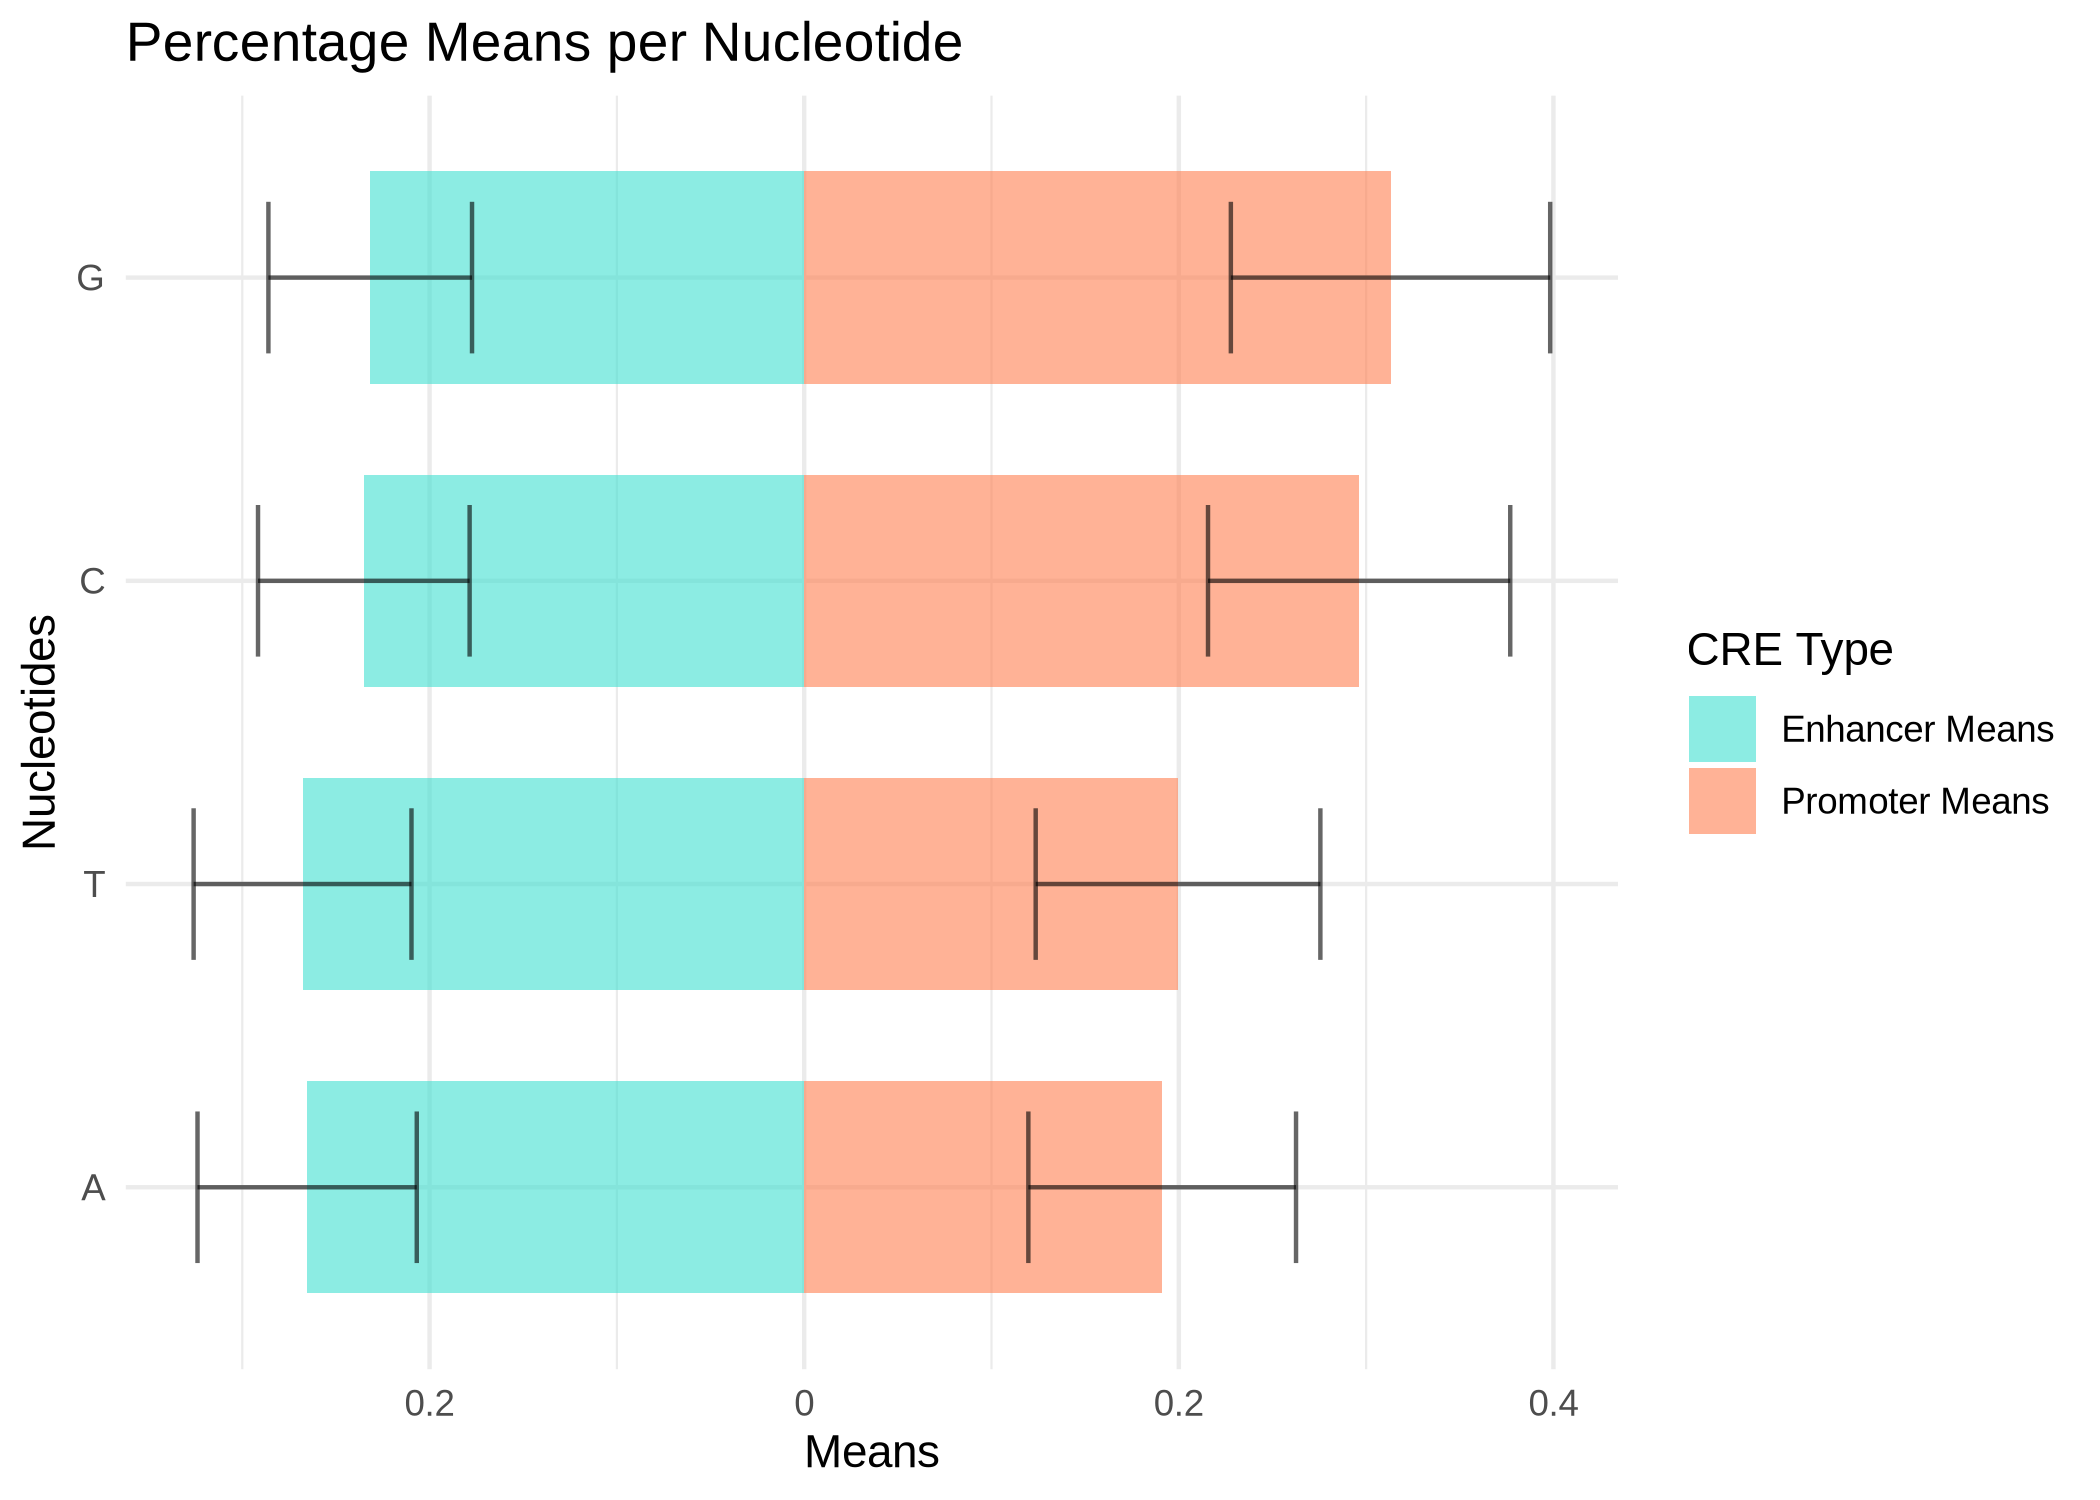
\includegraphics[width=\textwidth,height=1\textheight]{gb-test-pdf_files/figure-pdf/unnamed-chunk-21-1.png}
\end{center}

\begin{Shaded}
\begin{Highlighting}[]
\FunctionTok{library}\NormalTok{(cowplot)}

\NormalTok{temp\_plt }\OtherTok{\textless{}{-}} \FunctionTok{ggplot}\NormalTok{(subset\_cre\_temp) }\SpecialCharTok{+}
  \FunctionTok{geom\_bar}\NormalTok{(}\FunctionTok{aes}\NormalTok{(}\AttributeTok{x =} \FunctionTok{factor}\NormalTok{(Type), }
               \AttributeTok{y =}\NormalTok{ Means, }\AttributeTok{fill=}\NormalTok{Type),}
           \AttributeTok{stat =} \StringTok{"identity"}\NormalTok{, }\AttributeTok{position =} \StringTok{"identity"}\NormalTok{, }\AttributeTok{alpha =} \FloatTok{0.6}\NormalTok{) }\SpecialCharTok{+}
  \FunctionTok{geom\_errorbar}\NormalTok{(}\FunctionTok{aes}\NormalTok{(}\AttributeTok{x =} \FunctionTok{factor}\NormalTok{(Type), }
                    \AttributeTok{ymin =}\NormalTok{ Means }\SpecialCharTok{{-}}\NormalTok{ StDevs,}
                    \AttributeTok{ymax =}\NormalTok{ Means }\SpecialCharTok{+}\NormalTok{ StDevs),}
                \AttributeTok{width =} \FloatTok{0.5}\NormalTok{, }\AttributeTok{colour =} \StringTok{"black"}\NormalTok{, }\AttributeTok{alpha =} \FloatTok{0.6}\NormalTok{) }\SpecialCharTok{+}
  \FunctionTok{labs}\NormalTok{(}\AttributeTok{y =} \StringTok{"Means"}\NormalTok{, }\AttributeTok{x =} \StringTok{""}\NormalTok{, }
       \CommentTok{\# title = "Melting Temperature Means", }
       \AttributeTok{fill =} \StringTok{""}\NormalTok{) }\SpecialCharTok{+}
  \FunctionTok{scale\_y\_continuous}\NormalTok{(}\AttributeTok{breaks =} \FunctionTok{seq}\NormalTok{(}\DecValTok{0}\NormalTok{, }\DecValTok{100}\NormalTok{, }\DecValTok{10}\NormalTok{),}
                     \AttributeTok{labels =} \FunctionTok{seq}\NormalTok{(}\DecValTok{0}\NormalTok{, }\DecValTok{100}\NormalTok{, }\DecValTok{10}\NormalTok{)) }\SpecialCharTok{+}
  \FunctionTok{guides}\NormalTok{(}\AttributeTok{fill =} \StringTok{"none"}\NormalTok{) }\SpecialCharTok{+}
  \FunctionTok{theme\_minimal}\NormalTok{()}

\NormalTok{shan\_plt }\OtherTok{\textless{}{-}} \FunctionTok{ggplot}\NormalTok{(subset\_cre\_shan) }\SpecialCharTok{+}
  \FunctionTok{geom\_bar}\NormalTok{(}\FunctionTok{aes}\NormalTok{(}\AttributeTok{x =} \FunctionTok{factor}\NormalTok{(Type), }
               \AttributeTok{y =}\NormalTok{ Means, }\AttributeTok{fill=}\NormalTok{Type),}
           \AttributeTok{stat =} \StringTok{"identity"}\NormalTok{, }\AttributeTok{position =} \StringTok{"identity"}\NormalTok{, }\AttributeTok{alpha =} \FloatTok{0.6}\NormalTok{) }\SpecialCharTok{+}
  \FunctionTok{geom\_errorbar}\NormalTok{(}\FunctionTok{aes}\NormalTok{(}\AttributeTok{x =} \FunctionTok{factor}\NormalTok{(Type), }
                    \AttributeTok{ymin =}\NormalTok{ Means }\SpecialCharTok{{-}}\NormalTok{ StDevs,}
                    \AttributeTok{ymax =}\NormalTok{ Means }\SpecialCharTok{+}\NormalTok{ StDevs),}
                \AttributeTok{width =} \FloatTok{0.5}\NormalTok{, }\AttributeTok{colour =} \StringTok{"black"}\NormalTok{, }\AttributeTok{alpha =} \FloatTok{0.6}\NormalTok{) }\SpecialCharTok{+}
  \FunctionTok{labs}\NormalTok{(}\AttributeTok{y =} \StringTok{""}\NormalTok{, }\AttributeTok{x =} \StringTok{""}\NormalTok{, }
       \CommentTok{\# title = "Shannon Entropy Means", }
       \AttributeTok{fill =} \StringTok{"CRE Type"}\NormalTok{) }\SpecialCharTok{+}
  \FunctionTok{scale\_y\_continuous}\NormalTok{(}\AttributeTok{breaks=}\FunctionTok{seq}\NormalTok{(}\DecValTok{0}\NormalTok{, }\DecValTok{2}\NormalTok{, }\FloatTok{0.25}\NormalTok{), }\AttributeTok{labels=}\FunctionTok{seq}\NormalTok{(}\DecValTok{0}\NormalTok{, }\DecValTok{2}\NormalTok{, }\FloatTok{0.25}\NormalTok{)) }\SpecialCharTok{+}
  \FunctionTok{theme\_minimal}\NormalTok{()}

\FunctionTok{plot\_grid}\NormalTok{(temp\_plt, shan\_plt, }\AttributeTok{ncol =} \DecValTok{2}\NormalTok{, }\AttributeTok{rel\_widths =} \FunctionTok{c}\NormalTok{(}\DecValTok{1}\NormalTok{,}\FloatTok{1.5}\NormalTok{),}
          \AttributeTok{labels =} \FunctionTok{c}\NormalTok{(}\StringTok{"Melting Temperature"}\NormalTok{, }\StringTok{"Shannon Entropy"}\NormalTok{),}
          \AttributeTok{label\_fontface =} \StringTok{"plain"}\NormalTok{,}\AttributeTok{hjust =} \FunctionTok{c}\NormalTok{(}\SpecialCharTok{{-}}\FloatTok{0.35}\NormalTok{, }\SpecialCharTok{{-}}\FloatTok{0.48}\NormalTok{), }\AttributeTok{vjust =} \DecValTok{1}\NormalTok{)}
\end{Highlighting}
\end{Shaded}

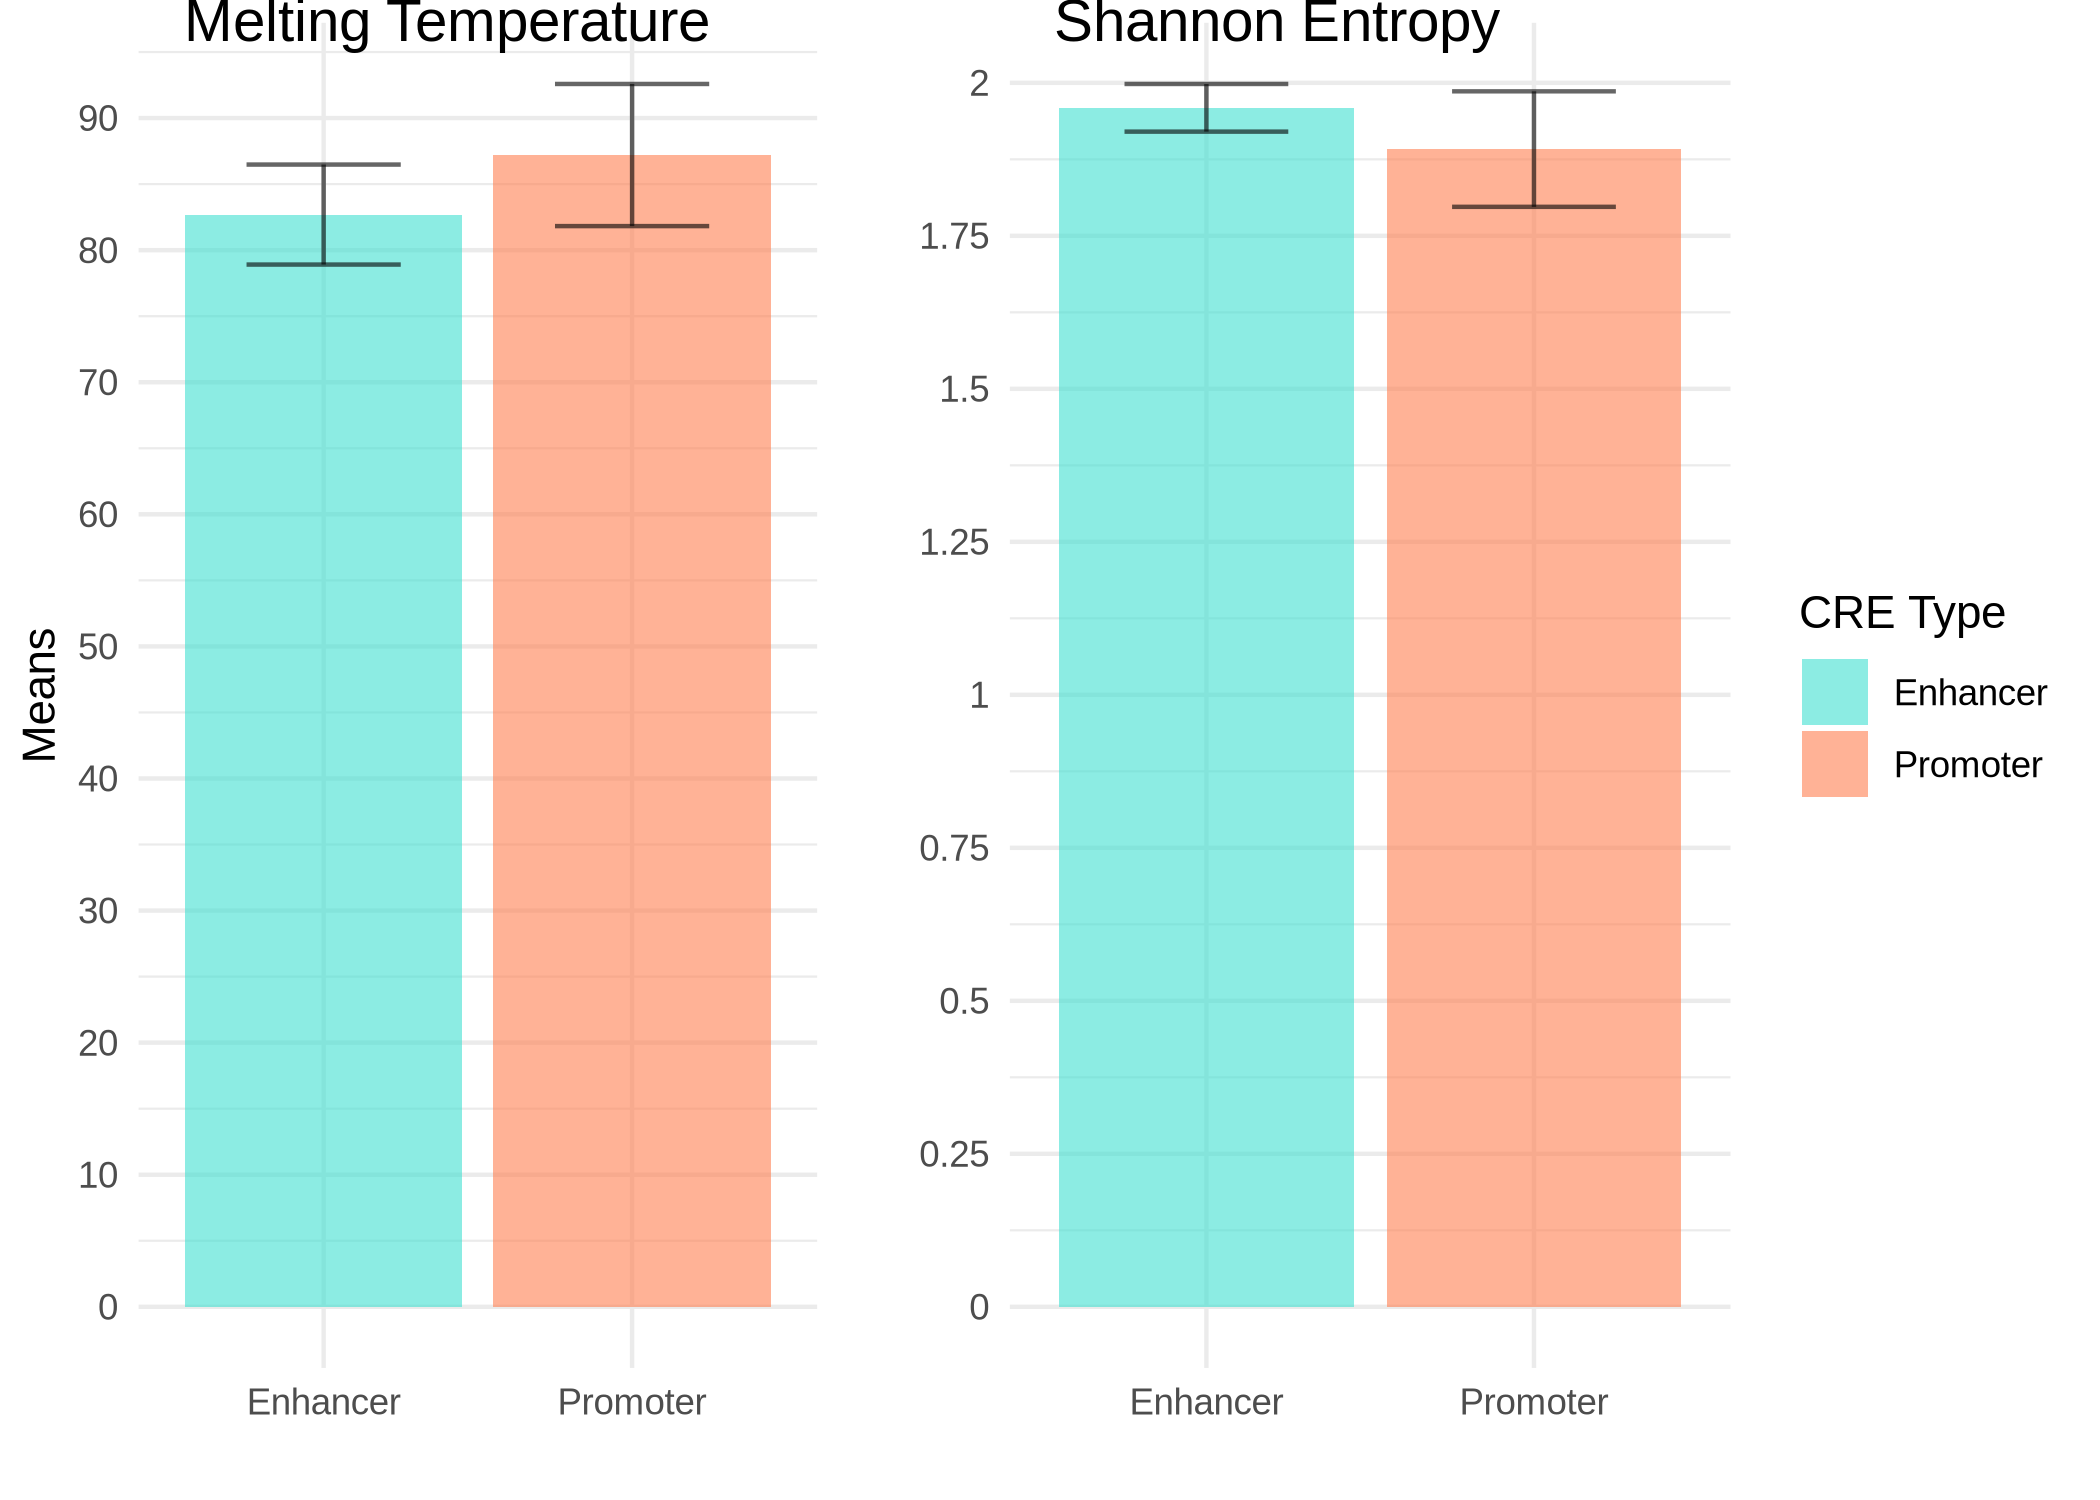
\includegraphics{gb-test-pdf_files/figure-pdf/unnamed-chunk-22-1.png}

\begin{Shaded}
\begin{Highlighting}[]
\FunctionTok{ggplot}\NormalTok{(subset\_cre\_prod) }\SpecialCharTok{+}
  \FunctionTok{geom\_bar}\NormalTok{(}\FunctionTok{aes}\NormalTok{(}\AttributeTok{x =} \FunctionTok{factor}\NormalTok{(Field, }\AttributeTok{levels =}\NormalTok{ field\_order\_prod), }
               \AttributeTok{y =} \FunctionTok{ifelse}\NormalTok{(Type }\SpecialCharTok{==} \StringTok{"Enhancer"}\NormalTok{, }\SpecialCharTok{{-}}\NormalTok{Means, Means), }
                          \AttributeTok{fill =} \FunctionTok{paste}\NormalTok{(Type, }\StringTok{"Means"}\NormalTok{)),}
               \AttributeTok{stat =} \StringTok{"identity"}\NormalTok{, }\AttributeTok{position =} \StringTok{"identity"}\NormalTok{, }
               \AttributeTok{alpha =} \FloatTok{0.6}\NormalTok{, }\AttributeTok{width =} \FloatTok{0.7}\NormalTok{) }\SpecialCharTok{+}
  \FunctionTok{geom\_errorbar}\NormalTok{(}\FunctionTok{aes}\NormalTok{(}\AttributeTok{x =} \FunctionTok{factor}\NormalTok{(Field, }\AttributeTok{levels =}\NormalTok{ field\_order\_prod),}
                    \AttributeTok{ymin =} \FunctionTok{ifelse}\NormalTok{(Type }\SpecialCharTok{==} \StringTok{"Enhancer"}\NormalTok{,}
                                  \SpecialCharTok{{-}}\NormalTok{Means }\SpecialCharTok{+}\NormalTok{ StDevs, Means }\SpecialCharTok{{-}}\NormalTok{ StDevs),}
                    \AttributeTok{ymax =} \FunctionTok{ifelse}\NormalTok{(Type }\SpecialCharTok{==} \StringTok{"Enhancer"}\NormalTok{,}
                                  \SpecialCharTok{{-}}\NormalTok{Means }\SpecialCharTok{{-}}\NormalTok{ StDevs, Means }\SpecialCharTok{+}\NormalTok{ StDevs)),}
                \AttributeTok{width =} \FloatTok{0.5}\NormalTok{, }\AttributeTok{colour =} \StringTok{"black"}\NormalTok{, }\AttributeTok{alpha =} \FloatTok{0.6}\NormalTok{) }\SpecialCharTok{+}
  \FunctionTok{coord\_flip}\NormalTok{() }\SpecialCharTok{+}
  \FunctionTok{scale\_y\_continuous}\NormalTok{(}\AttributeTok{breaks=}\FunctionTok{seq}\NormalTok{(}\SpecialCharTok{{-}}\DecValTok{30}\NormalTok{, }\DecValTok{30}\NormalTok{, }\DecValTok{10}\NormalTok{), }\AttributeTok{labels=}\FunctionTok{abs}\NormalTok{(}\FunctionTok{seq}\NormalTok{(}\SpecialCharTok{{-}}\DecValTok{30}\NormalTok{, }\DecValTok{30}\NormalTok{, }\DecValTok{10}\NormalTok{))) }\SpecialCharTok{+}
  \FunctionTok{scale\_fill\_manual}\NormalTok{(}\AttributeTok{values =} \FunctionTok{c}\NormalTok{(}\StringTok{"turquoise"}\NormalTok{, }\StringTok{"coral"}\NormalTok{)) }\SpecialCharTok{+}
  \FunctionTok{labs}\NormalTok{(}\AttributeTok{y =} \StringTok{"Means"}\NormalTok{, }\AttributeTok{x =} \StringTok{"Kmers"}\NormalTok{, }
       \AttributeTok{title =} \StringTok{"KSG{-}Product Means per Kmer"}\NormalTok{, }
       \AttributeTok{fill =} \StringTok{"CRE Type"}\NormalTok{) }\SpecialCharTok{+}
  \FunctionTok{theme\_minimal}\NormalTok{()}
\end{Highlighting}
\end{Shaded}

\begin{center}
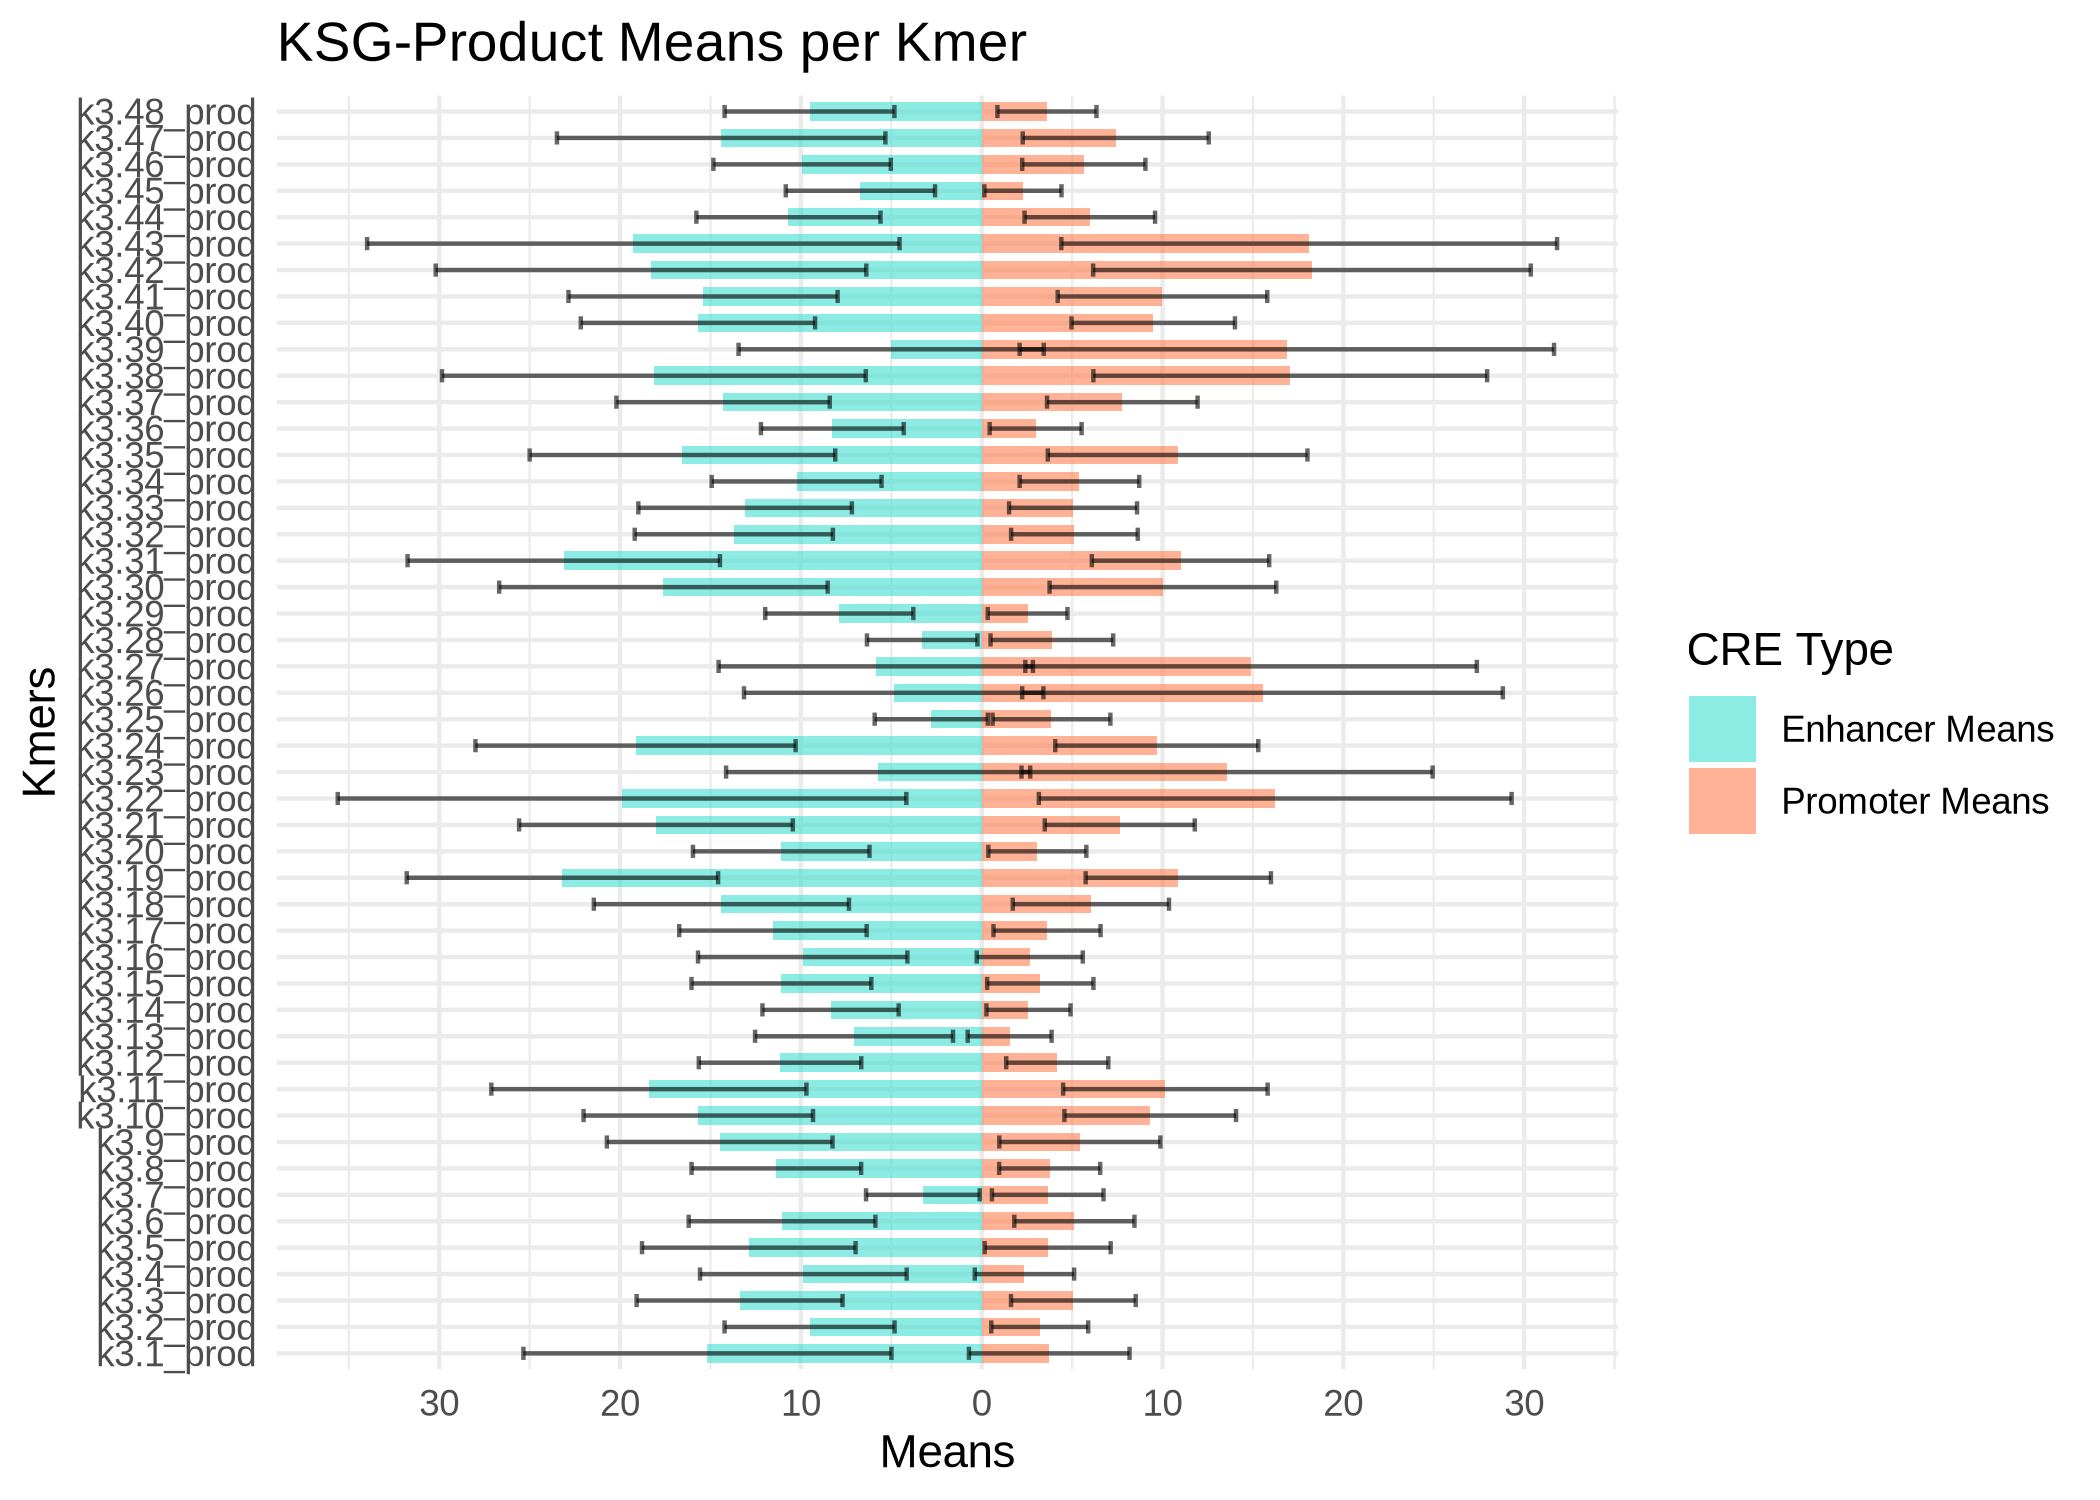
\includegraphics[width=\textwidth,height=1\textheight]{gb-test-pdf_files/figure-pdf/unnamed-chunk-23-1.png}
\end{center}

\begin{Shaded}
\begin{Highlighting}[]
\FunctionTok{ggplot}\NormalTok{(subset\_cre\_barc) }\SpecialCharTok{+}
  \FunctionTok{geom\_bar}\NormalTok{(}\FunctionTok{aes}\NormalTok{(}\AttributeTok{x =} \FunctionTok{factor}\NormalTok{(Field, }\AttributeTok{levels =}\NormalTok{ field\_order\_barc), }
               \AttributeTok{y =} \FunctionTok{ifelse}\NormalTok{(Type }\SpecialCharTok{==} \StringTok{"Enhancer"}\NormalTok{, }\SpecialCharTok{{-}}\NormalTok{Means, Means), }
                          \AttributeTok{fill =} \FunctionTok{paste}\NormalTok{(Type, }\StringTok{"Means"}\NormalTok{)),}
               \AttributeTok{stat =} \StringTok{"identity"}\NormalTok{, }\AttributeTok{position =} \StringTok{"identity"}\NormalTok{, }
               \AttributeTok{alpha =} \FloatTok{0.6}\NormalTok{, }\AttributeTok{width =} \FloatTok{0.7}\NormalTok{) }\SpecialCharTok{+}
  \FunctionTok{geom\_errorbar}\NormalTok{(}\FunctionTok{aes}\NormalTok{(}\AttributeTok{x =} \FunctionTok{factor}\NormalTok{(Field, }\AttributeTok{levels =}\NormalTok{ field\_order\_barc),}
                    \AttributeTok{ymin =} \FunctionTok{ifelse}\NormalTok{(Type }\SpecialCharTok{==} \StringTok{"Enhancer"}\NormalTok{,}
                                  \SpecialCharTok{{-}}\NormalTok{Means }\SpecialCharTok{+}\NormalTok{ StDevs, Means }\SpecialCharTok{{-}}\NormalTok{ StDevs),}
                    \AttributeTok{ymax =} \FunctionTok{ifelse}\NormalTok{(Type }\SpecialCharTok{==} \StringTok{"Enhancer"}\NormalTok{,}
                                  \SpecialCharTok{{-}}\NormalTok{Means }\SpecialCharTok{{-}}\NormalTok{ StDevs, Means }\SpecialCharTok{+}\NormalTok{ StDevs)),}
                \AttributeTok{width =} \FloatTok{0.5}\NormalTok{, }\AttributeTok{colour =} \StringTok{"black"}\NormalTok{, }\AttributeTok{alpha =} \FloatTok{0.6}\NormalTok{) }\SpecialCharTok{+}
  \FunctionTok{coord\_flip}\NormalTok{() }\SpecialCharTok{+}
  \FunctionTok{scale\_y\_continuous}\NormalTok{(}\AttributeTok{breaks=}\FunctionTok{seq}\NormalTok{(}\SpecialCharTok{{-}}\DecValTok{10}\NormalTok{, }\DecValTok{10}\NormalTok{, }\DecValTok{1}\NormalTok{), }\AttributeTok{labels=}\FunctionTok{abs}\NormalTok{(}\FunctionTok{seq}\NormalTok{(}\SpecialCharTok{{-}}\DecValTok{10}\NormalTok{, }\DecValTok{10}\NormalTok{, }\DecValTok{1}\NormalTok{))) }\SpecialCharTok{+}
  \FunctionTok{scale\_fill\_manual}\NormalTok{(}\AttributeTok{values =} \FunctionTok{c}\NormalTok{(}\StringTok{"turquoise"}\NormalTok{, }\StringTok{"coral"}\NormalTok{)) }\SpecialCharTok{+}
  \FunctionTok{labs}\NormalTok{(}\AttributeTok{y =} \StringTok{"Means"}\NormalTok{, }\AttributeTok{x =} \StringTok{"Kmers"}\NormalTok{, }
       \AttributeTok{title =} \StringTok{"Barcode Profile Means per Kmer"}\NormalTok{, }
       \AttributeTok{fill =} \StringTok{"CRE Type"}\NormalTok{) }\SpecialCharTok{+}
  \FunctionTok{theme\_minimal}\NormalTok{()}
\end{Highlighting}
\end{Shaded}

\begin{center}
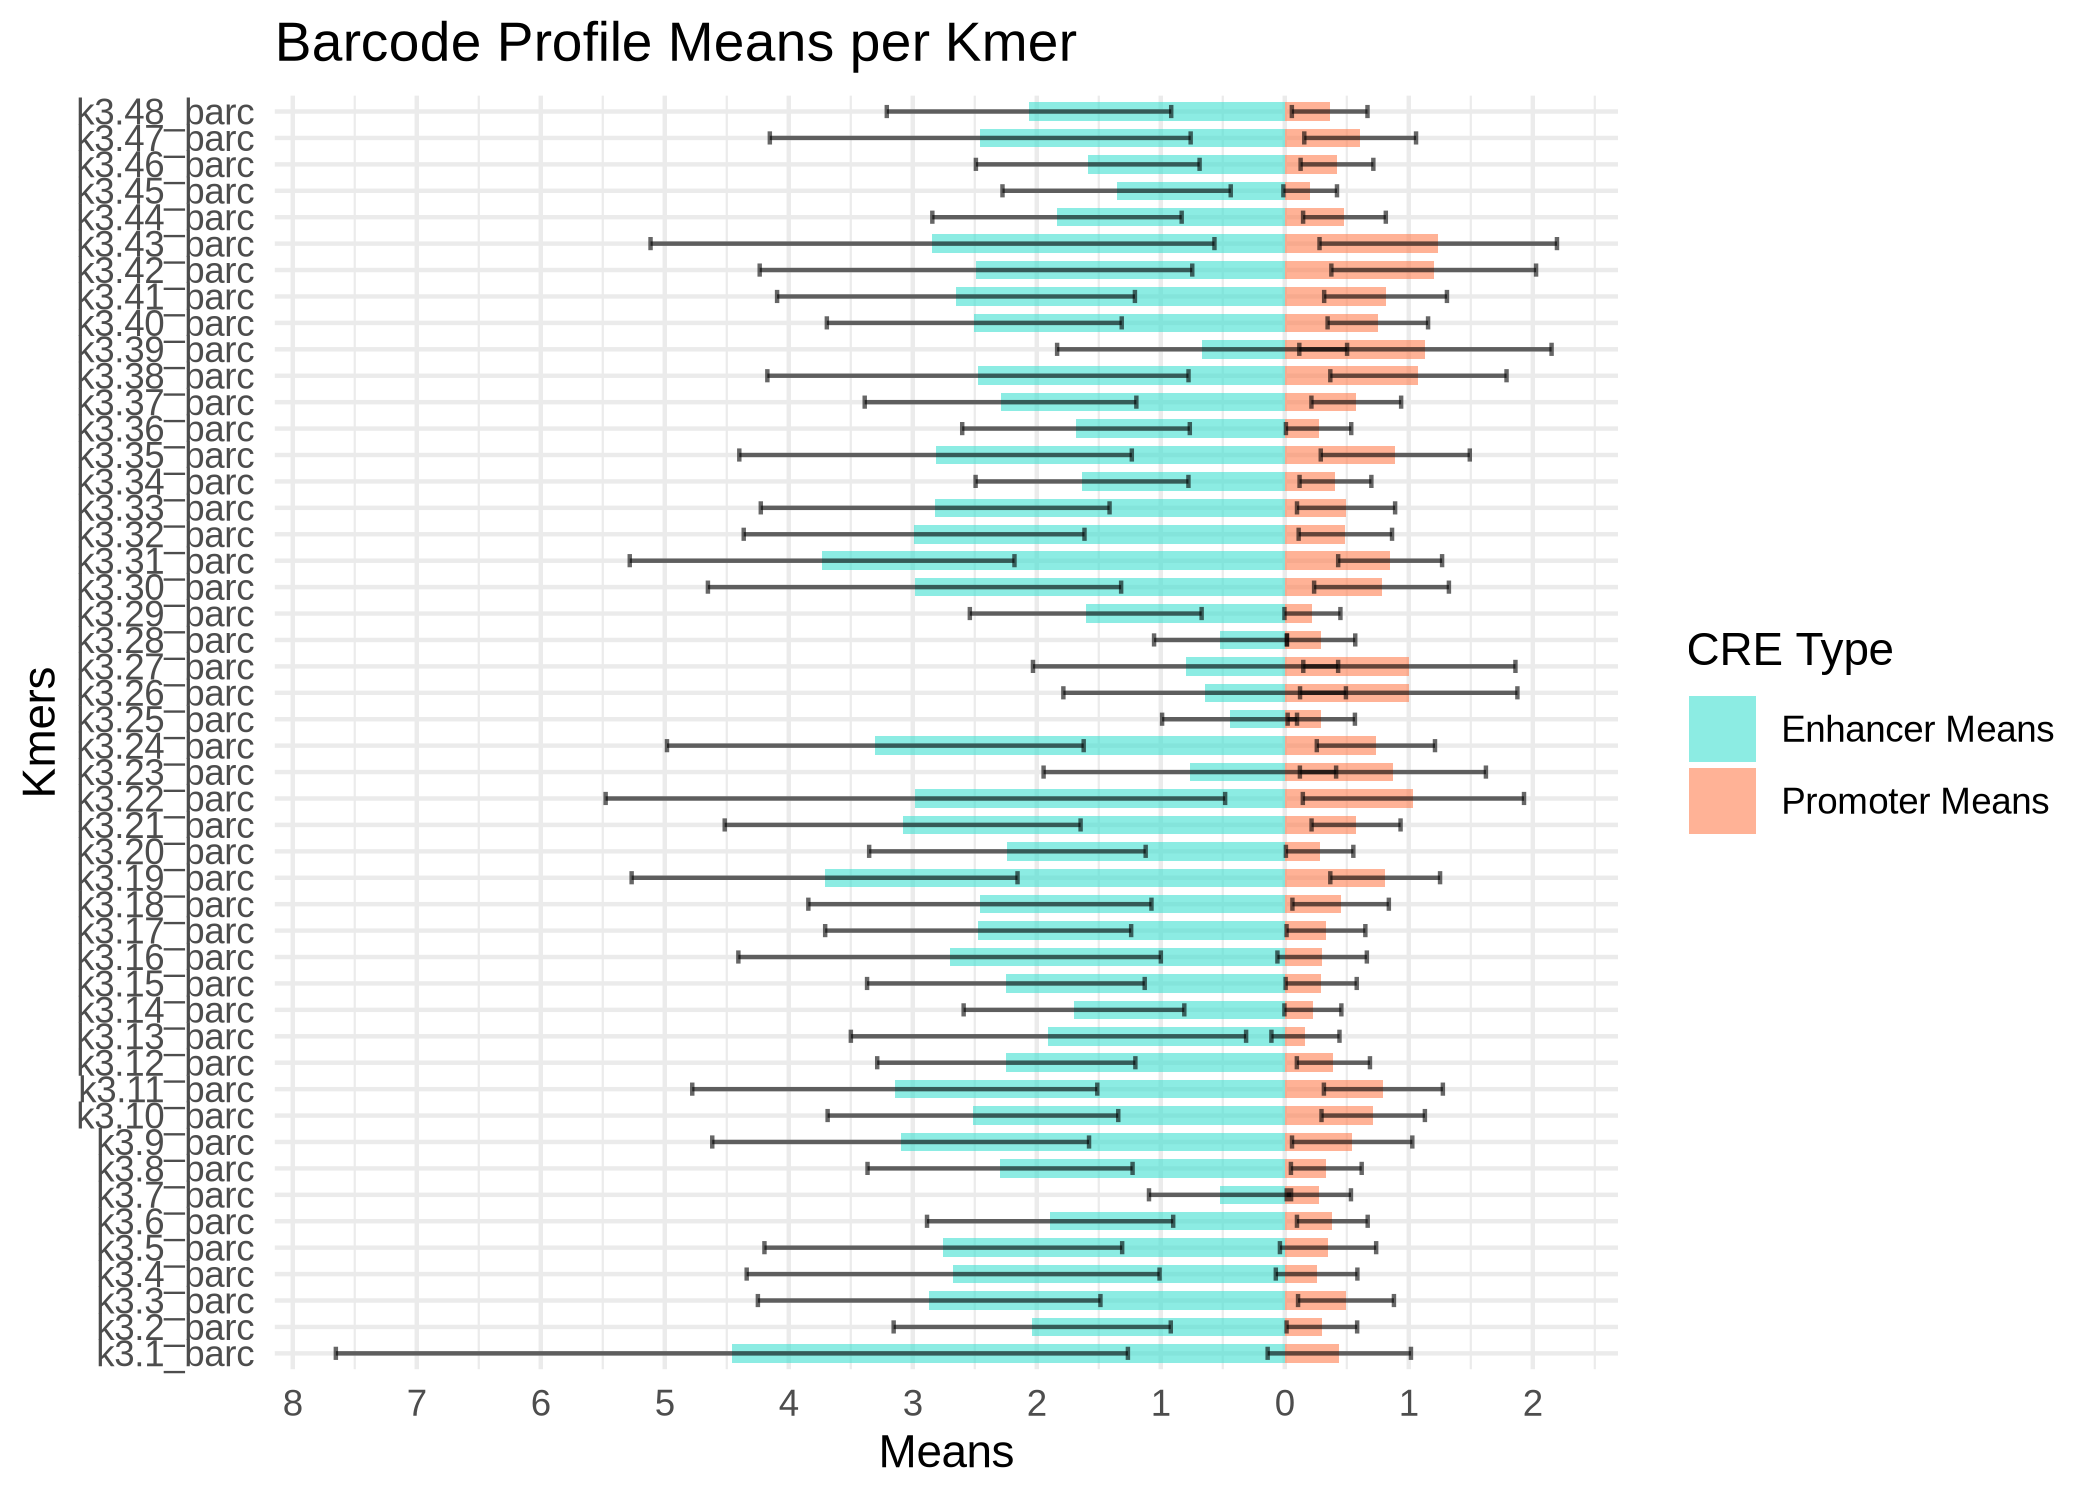
\includegraphics[width=\textwidth,height=1\textheight]{gb-test-pdf_files/figure-pdf/unnamed-chunk-24-1.png}
\end{center}



\end{document}
